% !TeX encoding = UTF-8
% !TeX program = xelatex
% !TeX spellcheck = en_US

\documentclass[degree=master]{thuthesis}
  % 学位 degree:
  %   doctor | master | bachelor | postdoc
  % 学位类型 degree-type:
  %   academic(默认)| professional


% 论文基本配置,加载宏包等全局配置
% !TeX root = ./thuthesis-example.tex

% 论文基本信息配置

\thusetup{
  %******************************
  % 注意:
  %   1. 配置里面不要出现空行
  %   2. 不需要的配置信息可以删除
  %   3. 建议先阅读文档中所有关于选项的说明
  %******************************
  %
  % 输出格式
  %   选择打印版(print)或用于提交的电子版(electronic),前者会插入空白页以便直接双面打印
  %
  output = print,
  %
  % 标题
  %   可使用“\\”命令手动控制换行
  %
  title  = { NVM 数据库的垃圾回收和数据恢复机制研究},
  title* = {Garbage Collection and Data Recovery for NVM-based Database},
  %
  % 学位
  %   1. 学术型
  %      - 中文
  %        需注明所属的学科门类,例如:
  %        哲学、经济学、法学、教育学、文学、历史学、理学、工学、农学、医学、
  %        军事学、管理学、艺术学
  %      - 英文
  %        博士:Doctor of Philosophy
  %        硕士:
  %          哲学、文学、历史学、法学、教育学、艺术学门类,公共管理学科
  %          填写“Master of Arts“,其它填写“Master of Science”
  %   2. 专业型
  %      直接填写专业学位的名称,例如:
  %      教育博士、工程硕士等
  %      Doctor of Education, Master of Engineering
  %   3. 本科生不需要填写
  %
  degree-name  = {工学硕士},
  degree-name* = {Master of Science},
  %
  % 培养单位
  %   填写所属院系的全名
  %
  department = {计算机科学与技术系},
  %
  % 学科
  %   1. 学术型学位
  %      获得一级学科授权的学科填写一级学科名称,其他填写二级学科名称
  %   2. 工程硕士
  %      工程领域名称
  %   3. 其他专业型学位
  %      不填写此项
  %   4. 本科生填写专业名称,第二学位论文需标注“(第二学位)”
  %
  discipline  = {计算机科学与技术},
  discipline* = {Computer Science and Technology},
  %
  % 姓名
  %
  author  = {蔡诗宇},
  author* = {Cai Shiyu},
  %
  % 指导教师
  %   中文姓名和职称之间以英文逗号“,”分开,下同
  %
  supervisor  = {武永卫, 教授},
  supervisor* = {Professor Wu Yongwei},
  %
  % 副指导教师
  %
  % associate-supervisor  = {陈康, 教授},
  % associate-supervisor* = {Professor Chen Kang},
  %
  % 联合指导教师
  %
  % joint-supervisor  = {某某某, 教授},
  % joint-supervisor* = {Professor Mou Moumou},
  %
  % 日期
  %   使用 ISO 格式;默认为当前时间
  %
  % date = {2019-07-07},
  %
  % 是否在中文封面后的空白页生成书脊(默认 false)
  %
  include-spine = false,
  %
  % 密级和年限
  %   秘密, 机密, 绝密
  %
  % secret-level = {秘密},
  % secret-year  = {10},
  %
  % 博士后专有部分
  %
  % clc                = {分类号},
  % udc                = {UDC},
  % id                 = {编号},
  % discipline-level-1 = {计算机科学与技术},  % 流动站(一级学科)名称
  % discipline-level-2 = {系统结构},          % 专业(二级学科)名称
  % start-date         = {2011-07-01},        % 研究工作起始时间
}

% 载入所需的宏包

% 可以使用 nomencl 生成符号和缩略语说明
% \usepackage{nomencl}
% \makenomenclature

% 表格加脚注
\usepackage{threeparttable}

% 表格中支持跨行
\usepackage{multirow}

% 固定宽度的表格。放在 hyperref 之前的话,tabularx 里的 footnote 显示不出来。
% \usepackage{tabularx}

% 跨页表格
% \usepackage{longtable}

% 量和单位
\usepackage{siunitx}

% 定理类环境宏包
\usepackage{amsthm}
% 也可以使用 ntheorem
% \usepackage[amsmath,thmmarks,hyperref]{ntheorem}

% 参考文献使用 BibTeX + natbib 宏包
% 顺序编码制
\usepackage[sort]{natbib}
\bibliographystyle{thuthesis-numeric}

% 著者-出版年制
% \usepackage{natbib}
% \bibliographystyle{thuthesis-author-year}

% 本科生参考文献的著录格式
% \usepackage[sort]{natbib}
% \bibliographystyle{thuthesis-bachelor}

% 参考文献使用 BibLaTeX 宏包
% \usepackage[backend=biber,style=thuthesis-numeric]{biblatex}
% \usepackage[backend=biber,style=thuthesis-author-year]{biblatex}
% \usepackage[backend=biber,style=apa]{biblatex}
% \usepackage[backend=biber,style=mla-new]{biblatex}
% 声明 BibLaTeX 的数据库
% \addbibresource{ref/refs.bib}

% 定义所有的图片文件在 figures 子目录下
\graphicspath{{figures/}}

% 数学命令
\newcommand\dif{\mathop{}\!\mathrm{d}}  % 微分符号

% hyperref 宏包在最后调用
\usepackage{hyperref}

% 算法生成
\usepackage[ruled,linesnumbered]{algorithm2e}


% 我的指令设置
% \renewcommand{\algorithmicrequire}{ \textbf{输入:}} %Use Input in the format of Algorithm
% \renewcommand{\algorithmicensure}{ \textbf{输出:}} %UseOutput in the format of Algorithm
\newcommand\todo[1]{\textcolor{red}{Todo: #1}}
\newcommand\INDSTATE{\ \ \ \ }

\begin{document}

% 封面
\maketitle

% 学位论文指导小组、公开评阅人和答辩委员会名单
% !TeX root = ../thuthesis-example.tex

\begin{committee}[name={学位论文指导小组、公开评阅人和答辩委员会名单}]

  \newcolumntype{C}[1]{@{}>{\centering\arraybackslash}p{#1}}

  \section*{指导小组名单}

  \begin{center}
    \begin{tabular}{C{3cm}C{3cm}C{9cm}@{}}
      李XX & 教授     & 清华大学 \\
      王XX & 副教授   & 清华大学 \\
      张XX & 助理教授 & 清华大学 \\
    \end{tabular}
  \end{center}


  \section*{公开评阅人名单}

  \begin{center}
    \begin{tabular}{C{3cm}C{3cm}C{9cm}@{}}
      刘XX & 教授   & 清华大学                    \\
      陈XX & 副教授 & XXXX大学                    \\
      杨XX & 研究员 & 中国XXXX科学院XXXXXXX研究所 \\
    \end{tabular}
  \end{center}


  \section*{答辩委员会名单}

  \begin{center}
    \begin{tabular}{C{2.75cm}C{2.98cm}C{4.63cm}C{4.63cm}@{}}
      主席 & 赵XX                  & 教授                    & 清华大学       \\
      委员 & 刘XX                  & 教授                    & 清华大学       \\
          & \multirow{2}{*}{杨XX} & \multirow{2}{*}{研究员} & 中国XXXX科学院 \\
          &                       &                         & XXXXXXX研究所  \\
          & 黄XX                  & 教授                    & XXXX大学       \\
          & 周XX                  & 副教授                  & XXXX大学       \\
      秘书 & 吴XX                  & 助理研究员              & 清华大学       \\
    \end{tabular}
  \end{center}

\end{committee}



% 也可以导入 Word 版转的 PDF 文件
% \begin{committee}[file=figures/committee.pdf]
% \end{committee}


% 使用授权的说明
\copyrightpage
% 将签字扫描后授权文件 scan-copyright.pdf 替换原始页面
% \copyrightpage[file=scan-copyright.pdf]

\frontmatter
% !TeX root = ../thuthesis-caishiyu.tex

% 中英文摘要和关键字

\begin{abstract}
    传统的数据库采用内存-非易失性介质的双层架构。
    数据库的数据有两份拷贝,一份在内存中作为高速的缓存,一份在非易失性介质上以保证数据非易失性。
    传统数据库的性能受限于双层介质之间的数据同步开销以及数据管理开销。

    非易失性内存(Non-Volatile Memory, NVM)是一种新的存储介质。
    NVM 支持字节寻址以及数据非易失性,同时其访问延迟与 DRAM 处于同一个数量级。
    NVM 硬件技术的商业化给数据库研究提供了新的方向,即采用单层存储架构。
    单层架构的数据库管理系统能够减少数据同步的开销,并使系统运行无日志化。

    然而无日志的前提给数据库的垃圾回收机制以及数据恢复机制带来了挑战。
    垃圾回收需要回收未被使用的空间。
    然而在无日志的前提下,数据管理无法保证分配空间以及使用空间的原子性,会造成持久化的内存泄漏问题。
    另一方面,数据库管理系统需要保证事务的原子性以及持久化,
    而日志文件记录了事务的操作。因此在恢复阶段,系统难以在无日志的前提下消除未提交事务的造成的片面影响。

    基于现有 NVM 工作的设计思路,本文设计了不基于日志系统的垃圾回收机制以及数据恢复机制。
    本文的主要贡献如下:
    \begin{enumerate}
        \item 本文采用了事务粒度的垃圾回收机制。在系统运行时,垃圾回收机制会尽可能地回收事务产生不可见的数据结构,以提高 NVM 存储空间的利用率。在恢复阶段,垃圾回收机制会回收泄漏的存储空间。
        \item 本文了结合了无日志的 NVM 分配器的设计思路,设计出第一个不基于日志的数据库恢复机制。本文通过设计 NVM 上数据结构来保证数据恢复时 NVM 数据的可读性。通过设计关键数据结构的可见性判断,系统能够在保证数据库 ACID 特性的前提下花费较低开销恢复到正常工作状态。
        \item 本文在 Intel Optane DC PMM 环境下测试了两种机制的效果。实验表明,垃圾回收机制能够在至多降低 $10\%$ 的运行时性能的前提下,帮助系统节约至多 $67\%$ 的存储空间。同时与 InnoDB 的恢复性能对比实验表明,本文所提出的无日志数据恢复机制的恢复时间十分迅速,1.5 GB 左右的记录数据仅需要 0.85 s 就能恢复成功。同时该恢复时间比基于写前日志的 InnoDB 的恢复时间低至多三个数量级。并且该数据恢复机制所使用的存储空间仅仅是 InnoDB 的一半。
    \end{enumerate}

    % 关键词用“英文逗号”分隔,输出时会自动处理为正确的分隔符
    \thusetup{
        keywords = {非易失性内存, 数据库管理系统, 垃圾回收, 数据恢复, 日志},
    }
\end{abstract}

\begin{abstract*}
    Traditional database management system (DBMS) uses a two-layer storage architecture.
    There are two copies of the record data, one in memory as a high-speed buffer and one in non-volatile storage to ensure data durability.
    The data synchronization overhead between the two storage and the complexity of data management are the bottlenecks of traditional databases.

    Non-volatile memory (NVM) supports byte-addressable memory access which is similar to DRAM, while at the same time, NVM can keep the
    in-memory data persistent like disks.
    The commercialization of NVM has provided a new direction for database research, namely the adoption of single-layer storage architecture.
    A single-layer architecture for database management systems can reduce the overhead of data synchronization and make the system run without logging.

    However, the log-freedom property poses a challenge to garbage collection  and data recovery of DBMS.
    With no logs, data management cannot guarantee the atomicity of memory allocation, which can lead to memory leaks.
    The memory leaks on NVM are persistent and are harmful to DBMS.
    On the other hand, the DBMS needs to ensure the atomicity and durability of transactions during the data recovery phase.
    The log file records the operation of the transaction. Thus, it is difficult for the system to eliminate the partial effects of uncommitted transactions without logging.

    Based on the design choices of existing NVM works, this paper presents garbage collection and data recovery for a log-freedom NVM-based DBMS.
    The main contributions of this paper are as follow:

    \begin{enumerate}
        \item This paper presents a transaction-level garbage collection that enables the DBMS to reclaim invisible data structures as soon as possible and saves NVM space. In the data recovery phase, the garbage collection reclaims the storage space to avoid potential memory leaks.
        \item This paper presents the first log-freedom data recovery mechanism which is based on the design choice of log-freedom NVM allocator. This paper ensures the readability of NVM data after reboot by designing the data structure on NVM. This paper also proposes visibility rules for key data structures. The rules enable the system to go back to work with less overhead while ensuring ACID properties.
        \item  This paper evaluates garbage collection and data recovery on Intel Optane DC PMM. The evaluation shows that enabling garbage collection results in up to
              10\% performance degradation, but saves up to 67\% storage space. Besides, our data recovery requires only 0.2\%
              of the time and half of the storage space of InnoDB.

    \end{enumerate}


    % Use comma as seperator when inputting
    \thusetup{
        keywords* = {Non-volatile memory, database management system, garbage collection, data recovery, log},
    }
\end{abstract*}


% 目录
\tableofcontents

% 插图和附表清单
\listoffiguresandtables  % 插图和附表清单
% \listoffigures           % 插图清单
% \listoftables            % 附表清单

% 符号对照表
% !TeX root = ../thuthesis-caishiyu.tex

\begin{denotation}[3cm]
  \item[PI] 聚酰亚胺
  \item[MPI] 聚酰亚胺模型化合物,N-苯基邻苯酰亚胺
  \item[PBI] 聚苯并咪唑
  \item[MPBI] 聚苯并咪唑模型化合物,N-苯基苯并咪唑
  \item[PY] 聚吡咙
  \item[PMDA-BDA] 均苯四酸二酐与联苯四胺合成的聚吡咙薄膜
  \item[MPY] 聚吡咙模型化合物
  \item[As-PPT] 聚苯基不对称三嗪
  \item[MAsPPT] 聚苯基不对称三嗪单模型化合物,3,5,6-三苯基-1,2,4-三嗪
  \item[DMAsPPT] 聚苯基不对称三嗪双模型化合物(水解实验模型化合物)
  \item[S-PPT] 聚苯基对称三嗪
  \item[MSPPT] 聚苯基对称三嗪模型化合物,2,4,6-三苯基-1,3,5-三嗪
  \item[PPQ] 聚苯基喹噁啉
  \item[MPPQ] 聚苯基喹噁啉模型化合物,3,4-二苯基苯并二嗪
  \item[HMPI] 聚酰亚胺模型化合物的质子化产物
  \item[HMPY] 聚吡咙模型化合物的质子化产物
  \item[HMPBI] 聚苯并咪唑模型化合物的质子化产物
  \item[HMAsPPT] 聚苯基不对称三嗪模型化合物的质子化产物
  \item[HMSPPT] 聚苯基对称三嗪模型化合物的质子化产物
  \item[HMPPQ] 聚苯基喹噁啉模型化合物的质子化产物
  \item[PDT] 热分解温度
  \item[HPLC] 高效液相色谱 (High Performance Liquid Chromatography)
  \item[HPCE] 高效毛细管电泳色谱 (High Performance Capillary lectrophoresis)
  \item[LC-MS] 液相色谱-质谱联用 (Liquid chromatography-Mass Spectrum)
  \item[TIC] 总离子浓度 (Total Ion Content)
  \item[\textit{ab initio}] 基于第一原理的量子化学计算方法,常称从头算法
  \item[DFT] 密度泛函理论 (Density Functional Theory)
  \item[$E_a$] 化学反应的活化能 (Activation Energy)
  \item[ZPE] 零点振动能 (Zero Vibration Energy)
  \item[PES] 势能面 (Potential Energy Surface)
  \item[TS] 过渡态 (Transition State)
  \item[TST] 过渡态理论 (Transition State Theory)
  \item[$\increment G^\neq$] 活化自由能(Activation Free Energy)
  \item[$\kappa$] 传输系数 (Transmission Coefficient)
  \item[IRC] 内禀反应坐标 (Intrinsic Reaction Coordinates)
  \item[$\nu_i$] 虚频 (Imaginary Frequency)
  \item[ONIOM] 分层算法 (Our own N-layered Integrated molecular Orbital and molecular Mechanics)
  \item[SCF] 自洽场 (Self-Consistent Field)
  \item[SCRF] 自洽反应场 (Self-Consistent Reaction Field)
\end{denotation}



% 也可以使用 nomencl 宏包,需要在导言区
% \usepackage{nomencl}
% \makenomenclature

% 在这里输出符号说明
% \printnomenclature[3cm]

% 在正文中的任意为都可以标题
% \nomenclature{PI}{聚酰亚胺}
% \nomenclature{MPI}{聚酰亚胺模型化合物,N-苯基邻苯酰亚胺}
% \nomenclature{PBI}{聚苯并咪唑}
% \nomenclature{MPBI}{聚苯并咪唑模型化合物,N-苯基苯并咪唑}
% \nomenclature{PY}{聚吡咙}
% \nomenclature{PMDA-BDA}{均苯四酸二酐与联苯四胺合成的聚吡咙薄膜}
% \nomenclature{MPY}{聚吡咙模型化合物}
% \nomenclature{As-PPT}{聚苯基不对称三嗪}
% \nomenclature{MAsPPT}{聚苯基不对称三嗪单模型化合物,3,5,6-三苯基-1,2,4-三嗪}
% \nomenclature{DMAsPPT}{聚苯基不对称三嗪双模型化合物(水解实验模型化合物)}
% \nomenclature{S-PPT}{聚苯基对称三嗪}
% \nomenclature{MSPPT}{聚苯基对称三嗪模型化合物,2,4,6-三苯基-1,3,5-三嗪}
% \nomenclature{PPQ}{聚苯基喹噁啉}
% \nomenclature{MPPQ}{聚苯基喹噁啉模型化合物,3,4-二苯基苯并二嗪}
% \nomenclature{HMPI}{聚酰亚胺模型化合物的质子化产物}
% \nomenclature{HMPY}{聚吡咙模型化合物的质子化产物}
% \nomenclature{HMPBI}{聚苯并咪唑模型化合物的质子化产物}
% \nomenclature{HMAsPPT}{聚苯基不对称三嗪模型化合物的质子化产物}
% \nomenclature{HMSPPT}{聚苯基对称三嗪模型化合物的质子化产物}
% \nomenclature{HMPPQ}{聚苯基喹噁啉模型化合物的质子化产物}
% \nomenclature{PDT}{热分解温度}
% \nomenclature{HPLC}{高效液相色谱 (High Performance Liquid Chromatography)}
% \nomenclature{HPCE}{高效毛细管电泳色谱 (High Performance Capillary lectrophoresis)}
% \nomenclature{LC-MS}{液相色谱-质谱联用 (Liquid chromatography-Mass Spectrum)}
% \nomenclature{TIC}{总离子浓度 (Total Ion Content)}
% \nomenclature{\textit{ab initio}}{基于第一原理的量子化学计算方法,常称从头算法}
% \nomenclature{DFT}{密度泛函理论 (Density Functional Theory)}
% \nomenclature{$E_a$}{化学反应的活化能 (Activation Energy)}
% \nomenclature{ZPE}{零点振动能 (Zero Vibration Energy)}
% \nomenclature{PES}{势能面 (Potential Energy Surface)}
% \nomenclature{TS}{过渡态 (Transition State)}
% \nomenclature{TST}{过渡态理论 (Transition State Theory)}
% \nomenclature{$\increment G^\neq$}{活化自由能(Activation Free Energy)}
% \nomenclature{$\kappa$}{传输系数 (Transmission Coefficient)}
% \nomenclature{IRC}{内禀反应坐标 (Intrinsic Reaction Coordinates)}
% \nomenclature{$\nu_i$}{虚频 (Imaginary Frequency)}
% \nomenclature{ONIOM}{分层算法 (Our own N-layered Integrated molecular Orbital and molecular Mechanics)}
% \nomenclature{SCF}{自洽场 (Self-Consistent Field)}
% \nomenclature{SCRF}{自洽反应场 (Self-Consistent Reaction Field)}



% 正文部分
\mainmatter
% % !TeX root = ../thuthesis-caishiyu.tex

\chapter{论文主要部分的写法}

研究生学位论文撰写,除表达形式上需要符合一定的格式要求外,内容方面上也要遵循一些共性原则。

通常研究生学位论文只能有一个主题(不能是几块工作拼凑在一起),该主题应针对某学科领域中的一个具体问题展开深入、系统的研究,并得出有价值的研究结论。
学位论文的研究主题切忌过大,例如,“中国国有企业改制问题研究”这样的研究主题过大,因为“国企改制”涉及的问题范围太广,很难在一本研究生学位论文中完全研究透彻。



\section{论文的语言及表述}

除国际研究生外,学位论文一律须用汉语书写。
学位论文应当用规范汉字进行撰写,除古汉语研究中涉及的古文字和参考文献中引用的外文文献之外,均采用简体汉字撰写。

国际研究生一般应以中文或英文书写学位论文,格式要求同上。
论文须用中文封面。

研究生学位论文是学术作品,因此其表述要严谨简明,重点突出,专业常识应简写或不写,做到立论正确、数据可靠、说明透彻、推理严谨、文字凝练、层次分明,避免使用文学性质的或带感情色彩的非学术性语言。

论文中如出现一个非通用性的新名词、新术语或新概念,需随即解释清楚。



\section{论文题目的写法}

论文题目应简明扼要地反映论文工作的主要内容,力求精炼、准确,切忌笼统。
论文题目是对研究对象的准确、具体描述,一般要在一定程度上体现研究结论,因此,论文题目不仅应告诉读者这本论文研究了什么问题,更要告诉读者这个研究得出的结论。
例如:“在事实与虚构之间:梅乐、卡彭特、沃尔夫的新闻观”就比“三个美国作家的新闻观研究”更专业、更准确。



\section{摘要的写法}

论文摘要是对论文研究内容的高度概括,应具有独立性和自含性,即应是 一篇简短但意义完整的文章。
通过阅读论文摘要,读者应该能够对论文的研究 方法及结论有一个整体性的了解,因此摘要的写法应力求精确简明。
论文摘要 应包括对问题及研究目的的描述、对使用的方法和研究过程进行的简要介绍、 对研究结论的高度凝练等,重点是结果和结论。

论文摘要切忌写成全文的提纲,尤其要避免“第 1 章……;第 2 章……;……”这样的陈述方式。



\section{引言的写法}

一篇学位论文的引言大致包含如下几个部分:
1、问题的提出;
2、选题背 景及意义;
3、文献综述;
4、研究方法;
5、论文结构安排。
\begin{itemize}
  \item 问题的提出:要清晰地阐述所要研究的问题“是什么”。
        \footnote{选题时切记要有“问题意识”,不要选不是问题的问题来研究。}
  \item 选题背景及意义:论述清楚为什么选择这个题目来研究,即阐述该研究对学科发展的贡献、对国计民生的理论与现实意义等。
  \item 文献综述:对本研究主题范围内的文献进行详尽的综合述评,“述”的同时一定要有“评”,指出现有研究状态,仍存在哪些尚待解决的问题,讲出自己的研究有哪些探索性内容。
  \item 研究方法:讲清论文所使用的学术研究方法。
  \item 论文结构安排:介绍本论文的写作结构安排。
\end{itemize}



\section{正文的写法}

本部分是论文作者的研究内容,不能将他人研究成果不加区分地掺和进来。
已经在引言的文献综述部分讲过的内容,这里不需要再重复。
各章之间要存在有机联系,符合逻辑顺序。



\section{结论的写法}

结论是对论文主要研究结果、论点的提炼与概括,应精炼、准确、完整,使读者看后能全面了解论文的意义、目的和工作内容。
结论是最终的、总体的结论,不是正文各章小结的简单重复。
结论应包括论文的核心观点,主要阐述作者的创造性工作及所取得的研究成果在本领域中的地位、作用和意义,交代研究工作的局限,提出未来工作的意见或建议。
同时,要严格区分自己取得的成果与指导教师及他人的学术成果。

在评价自己的研究工作成果时,要实事求是,除非有足够的证据表明自己的研究是“首次”、“领先”、“填补空白”的,否则应避免使用这些或类似词语。

% % !TeX root = ../thuthesis-caishiyu.tex

\chapter{图表示例}

\section{插图}

图片通常在 \env{figure} 环境中使用 \cs{includegraphics} 插入,如图~\ref{fig:example} 的源代码。
建议矢量图片使用 PDF 格式,比如数据可视化的绘图;
照片应使用 JPG 格式;
其他的栅格图应使用无损的 PNG 格式。
注意,LaTeX 不支持 TIFF 格式;EPS 格式已经过时。

\begin{figure}
  \centering
  
\includegraphics[width=0.6\linewidth]{example-image-a.pdf}
  \caption{示例图片}
  \label{fig:example}
\end{figure}

若图或表中有附注,采用英文小写字母顺序编号,附注写在图或表的下方。
% LaTeX 传统上一般将附注的内容同图表的标题写在一起,形成很长的一段文字。

如果一个图由两个或两个以上分图组成时,各分图分别以(a)、(b)、(c)...... 作为图序,并须有分图题。
推荐使用 \pkg{subcaption} 宏包来处理, 比如图~\ref{fig:subfig-a} 和图~\ref{fig:subfig-b}。

\begin{figure}
  \centering
  \subcaptionbox{分图 A\label{fig:subfig-a}}
  {
\includegraphics[width=0.45\linewidth]{example-image-a.pdf}}
  \subcaptionbox{分图 B\label{fig:subfig-b}}
  {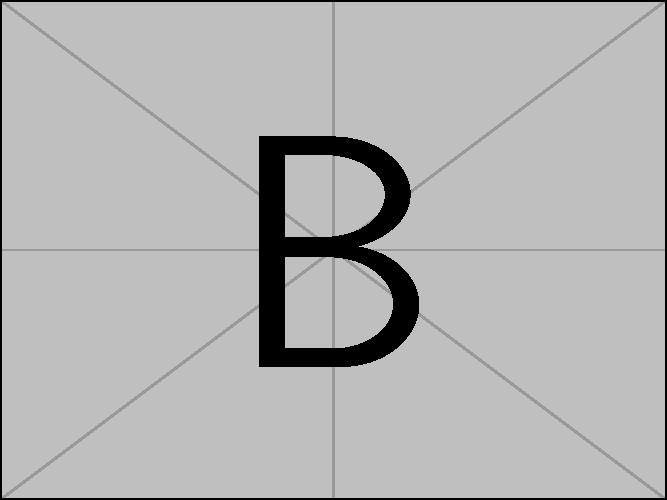
\includegraphics[width=0.45\linewidth]{example-image-b.pdf}}
  \caption{多个分图的示例}
  \label{fig:multi-image}
\end{figure}



\section{表格}

表应具有自明性。为使表格简洁易读,尽可能采用三线表,如表~\ref{tab:three-line}。
三条线可以使用 \pkg{booktabs} 宏包提供的命令生成。

\begin{table}
  \centering
  \caption{三线表示例}
  \begin{tabular}{ll}
    \toprule
    文件名          & 描述                         \\
    \midrule
    thuthesis.dtx   & 模板的源文件,包括文档和注释 \\
    thuthesis.cls   & 模板文件                     \\
    thuthesis-*.bst & BibTeX 参考文献表样式文件    \\
    thuthesis-*.bbx & BibLaTeX 参考文献表样式文件  \\
    thuthesis-*.cbx & BibLaTeX 引用样式文件        \\
    \bottomrule
  \end{tabular}
  \label{tab:three-line}
\end{table}

表格如果有附注,尤其是需要在表格中进行标注时,可以使用 \pkg{threeparttable} 宏包。
研究生要求使用英文小写字母 a、b、c……顺序编号,本科生使用圈码 ①、②、③……编号。

\begin{table}
  \centering
  \begin{threeparttable}[c]
    \caption{带附注的表格示例}
    \label{tab:three-part-table}
    \begin{tabular}{ll}
      \toprule
      文件名                 & 描述                         \\
      \midrule
      thuthesis.dtx\tnote{a} & 模板的源文件,包括文档和注释 \\
      thuthesis.cls\tnote{b} & 模板文件                     \\
      thuthesis-*.bst        & BibTeX 参考文献表样式文件    \\
      thuthesis-*.bbx        & BibLaTeX 参考文献表样式文件  \\
      thuthesis-*.cbx        & BibLaTeX 引用样式文件        \\
      \bottomrule
    \end{tabular}
    \begin{tablenotes}
      \item [a] 可以通过 xelatex 编译生成模板的使用说明文档;
      使用 xetex 编译 \file{thuthesis.ins} 时则会从 \file{.dtx} 中去除掉文档和注释,得到精简的 \file{.cls} 文件。
      \item [b] 更新模板时,一定要记得编译生成 \file{.cls} 文件,否则编译论文时载入的依然是旧版的模板。
    \end{tablenotes}
  \end{threeparttable}
\end{table}

% % !TeX root = ../thuthesis-example.tex

\chapter{数学符号和公式}

\section{数学符号}

研究生《写作指南》要求量及其单位所使用的符号应符合国家标准《国际单位制及其应用》(GB 3100—1993)、《有关量、单位和符号的一般原则》(GB/T 3101—1993) 的规定。
模板中使用 \pkg{unicode-math} 宏包来配置数学符号,
与 \LaTeX{} 默认的英美国家的符号习惯有所差异:
\begin{enumerate}
  \item 大写希腊字母默认为斜体,如 \cs{Delta}:$\Delta$。
  \item 有限增量符号 $\increment$(U+2206)应使用 \pkg{unicode-math} 宏包提供的
    \cs{increment} 命令。
  \item 向量、矩阵和张量要求粗斜体,应该使用 \pkg{unicode-math} 的 \cs{symbf} 命令,
    如 \verb|\symbf{A}|、\verb|\symbf{\alpha}|。
  \item 数学常数和特殊函数要求用正体,应使用 \cs{symup} 命令,
    如 $\symup{\pi} = 3.14\dots$; $\symup{e} = 2.718\dots$,
  \item 微分号和积分号使用使用正体,比如 $\int f(x) \dif x$。
\end{enumerate}

关于数学符号更多的用法,参考
\href{http://mirrors.ctan.org/macros/latex/contrib/unicode-math/unicode-math.pdf}{\pkg{unicode-math}}
宏包的使用说明,
全部数学符号命的令参考
\href{http://mirrors.ctan.org/macros/latex/contrib/unicode-math/unimath-symbols.pdf}{\pkg{unimath-symbols}}。

关于量和单位推荐使用
\href{http://mirrors.ctan.org/macros/latex/contrib/siunitx/siunitx.pdf}{\pkg{siunitx}}
宏包,
可以方便地处理希腊字母以及数字与单位之间的空白,
比如:
\SI{6.4e6}{m},
\SI{9}{\micro\meter},
\si{kg.m.s^{-1}},
\SIrange{10}{20}{\degreeCelsius}。



\section{数学公式}

数学公式可以使用 \env{equation} 和 \env{equation*} 环境。
注意数学公式的引用应前后带括号,建议使用 \cs{eqref} 命令,比如式 \eqref{eq:example}。
\begin{equation}
  \frac{1}{2 \symup{\pi} \symup{i}} \int_\gamma f = \sum_{k=1}^m n(\gamma; a_k) \mathscr{R}(f; a_k)
  \label{eq:example}
\end{equation}
注意公式编号的引用应含有圆括号,可以使用 \cs{eqref} 命令。

多行公式尽可能在“=”处对齐,推荐使用 \env{align} 环境。
\begin{align}
  a & = b + c + d + e \\
    & = f + g
\end{align}



\section{数学定理}

定理环境的格式可以使用 \pkg{amsthm} 或者 \pkg{ntheorem} 宏包配置。
用户在导言区载入这两者之一后,模板会自动配置 \env{thoerem}、\env{proof} 等环境。

\begin{theorem}[Lindeberg--Lévy 中心极限定理]
  设随机变量 $X_1, X_2, \dots, X_n$ 独立同分布, 且具有期望 $\mu$ 和有限的方差 $\sigma^2 \ne 0$,
  记 $\bar{X}_n = \frac{1}{n} \sum_{i+1}^n X_i$,则
  \begin{equation}
    \lim_{n \to \infty} P \left(\frac{\sqrt{n} \left( \bar{X}_n - \mu \right)}{\sigma} \le z \right) = \Phi(z),
  \end{equation}
  其中 $\Phi(z)$ 是标准正态分布的分布函数。
\end{theorem}
\begin{proof}
  Trivial.
\end{proof}

同时模板还提供了 \env{assumption}、\env{definition}、\env{proposition}、
\env{lemma}、\env{theorem}、\env{axiom}、\env{corollary}、\env{exercise}、
\env{example}、\env{remar}、\env{problem}、\env{conjecture} 这些相关的环境。

% % !TeX root = ../thuthesis-caishiyu.tex

\chapter{引用文献的标注}

模板支持 BibTeX 和 BibLaTeX 两种方式处理参考文献。
下文主要介绍 BibTeX 配合 \pkg{natbib} 宏包的主要使用方法。


\section{顺序编码制}

在顺序编码制下,默认的 \cs{cite} 命令同 \cs{citep} 一样,序号置于方括号中,
引文页码会放在括号外。
统一处引用的连续序号会自动用短横线连接。

\thusetup{
  cite-style = super,
}
\begin{tabular}{l@{\quad$\Rightarrow$\quad}l}
  \verb|\cite{zhangkun1994}| & \cite{zhangkun1994}               \\
  \verb|\citet{zhangkun1994}| & \citet{zhangkun1994}              \\
  \verb|\citep{zhangkun1994}| & \citep{zhangkun1994}              \\
  \verb|\cite[42]{zhangkun1994}| & \cite[42]{zhangkun1994}           \\
  \verb|\cite{zhangkun1994,zhukezhen1973}| & \cite{zhangkun1994,zhukezhen1973} \\
\end{tabular}


也可以取消上标格式,将数字序号作为文字的一部分。
建议全文统一使用相同的格式。

\thusetup{
  cite-style = inline,
}
\begin{tabular}{l@{\quad$\Rightarrow$\quad}l}
  \verb|\cite{zhangkun1994}|  & \cite{zhangkun1994}               \\
  \verb|\citet{zhangkun1994}|  & \citet{zhangkun1994}              \\
  \verb|\citep{zhangkun1994}|  & \citep{zhangkun1994}              \\
  \verb|\cite[42]{zhangkun1994}|  & \cite[42]{zhangkun1994}           \\
  \verb|\cite{zhangkun1994,zhukezhen1973}| & \cite{zhangkun1994,zhukezhen1973} \\
\end{tabular}



\section{著者-出版年制}

著者-出版年制下的 \cs{cite} 跟 \cs{citet} 一样。

\thusetup{
  cite-style = author-year,
}
\begin{tabular}{l@{\quad$\Rightarrow$\quad}l}
  \verb|\cite{zhangkun1994}| & \cite{zhangkun1994}                \\
  \verb|\citet{zhangkun1994}| & \citet{zhangkun1994}               \\
  \verb|\citep{zhangkun1994}| & \citep{zhangkun1994}               \\
  \verb|\cite[42]{zhangkun1994}| & \cite[42]{zhangkun1994}            \\
  \verb|\citep{zhangkun1994,zhukezhen1973}| & \citep{zhangkun1994,zhukezhen1973} \\
\end{tabular}

\vskip 2ex
\thusetup{
  cite-style = super,
}
注意,引文参考文献的每条都要在正文中标注
\cite{zhangkun1994,zhukezhen1973,dupont1974bone,zhengkaiqing1987,%
  jiangxizhou1980,jianduju1994,merkt1995rotational,mellinger1996laser,%
  bixon1996dynamics,mahui1995,carlson1981two,taylor1983scanning,%
  taylor1981study,shimizu1983laser,atkinson1982experimental,%
  kusch1975perturbations,guangxi1993,huosini1989guwu,wangfuzhi1865songlun,%
  zhaoyaodong1998xinshidai,biaozhunhua2002tushu,chubanzhuanye2004,%
  who1970factors,peebles2001probability,baishunong1998zhiwu,%
  weinstein1974pathogenic,hanjiren1985lun,dizhi1936dizhi,%
  tushuguan1957tushuguanxue,aaas1883science,fugang2000fengsha,%
  xiaoyu2001chubanye,oclc2000about,scitor2000project%
}。


% !TeX root = ../thuthesis-caishiyu.tex

\chapter{引言}

\section{研究意义}

在大数据的趋势下,一个能够支持大量数据,大量用户的高性能的数据库管理系统(Database Management System,DBMS)至关重要。传统的 DBMS 是基于两层存储结构,一层是内存(DRAM),而另一层是非易失性存储介质,例如硬盘(Hard Disk Drive,HDD)和固态硬盘(Solid-State Disk,SSD)。数据库可以根据数据的主要存储介质分成两类,磁盘数据库(Disk-Oriented Database)以及内存数据库(In-Memory Database)。
磁盘数据库将非易失性存储介质的数据拷贝到内存中作为数据缓存,以方便事务访问。
内存数据库则是将数据主要存储在内存中,将日志和检查点存储在非易失性存储介质以保证数据持久化。
这两类数据库的共同点在于,数据在内存中被访问读写。系统需要将事务对数据的影响以某种形式持久化到非易失性介质。
但是非易失性介质的访问速度与内存的访问速度之间存在巨大的鸿沟,因此频繁地进行数据持久化会降低数据库管理系统的性能。

非易失性内存(Non-Volatile Memory,NVM)是一种新的硬件存储技术。NVM 结合了 DRAM 以及 SSD 的优势。非易失性内存既像内存一样支持低延迟的字节寻址的数据访问,也和磁盘一样是一个大容量的非易失性介质。NVM 的出现给数据库管理系统的研究提供了一种新的方向。
现有的 NVM 数据库工作的设计方法有三类。
一类 NVM 数据库研究使用 NVM 替换数据库的存储介质\cite{arulraj_lets_2015, van_renen_managing_2018,mariaDB}。由于 NVM 的访问性能相较于磁盘的访问性能更为优异,此类方法能带来性能的提升。
另一类则是局部重新设计以追求局部的性能提升。Facebook 使用 NVM 降低存储的成本\cite{facebook},SAP HANA 则使用 NVM 存放一部分数据来降低恢复时间\cite{andrei_sap_2017}。
另外一些工作针对 NVM 的特性重新设计数据库的组件,例如事务引擎\cite{liu2018dudetx},索引\cite{nv-tree,chen_persistent_2015,ma_roart_2021,arulraj2018bztree},日志\cite{wbl}以及分配器\cite{pmdk,bhandari_makalu_2016}等。
前两种设计方法仍停留在传统数据库的设计框架中。此类系统仍使用复杂的数据管理机制以及日志系统来填补两个介质之间的性能差异。
第三种思路是整体重新设计架构,比如 N2DB\cite{liu_graduate_chinese} 和 Zen\cite{liu_zen_2021}。二者利用 NVM 的特性,设计了无日志的数据库系统。
无日志的特性减少系统在运行时由于数据同步以及数据管理的开销,提高了系统的性能。

现有 NVM 相关研究也在尝试无日志化或者少日志化。
NVM 事务内存只需要采用重做日志(Redo Log)或者回滚日志(Undo Log)的一种\cite{coburn_nv-heaps_2011, kolli_high-performance_2016,volos_mnemosyne_2011, giles_softwrap_2015, giles2017continuous}。
而 NVM 分配器能够实现彻底的无日志化\cite{bhandari_makalu_2016,cai_understanding_2020}。
无日志的 NVM 分配器不保证数据分配的原子性,因此宕机会造成内存泄漏问题。
此类 NVM 分配器的解决方法是通过数据结构的设计来保证分配器能够在重启后找到所有被使用的空间,并且使用垃圾回收机制异步地清理内存泄漏的空间。
该方法被称之为懒惰垃圾回收(Lazy Garbage Collection)。懒惰垃圾回收的核心在于将运行时的日志系统开销转化成恢复时的垃圾回收开销。

无日志的 NVM 数据库相对于无日志的 NVM 分配器更加复杂,其既要解决内存泄漏问题,也要保证事务满足 ACID (原子性,一致性,隔离性以及持久化)四个特性。
垃圾回收和数据恢复是数据库解决上述问题的途径。
垃圾回收机制负责在运行时回收不被使用的空间,在恢复时回收内存泄漏的空间。数据恢复机制负责在宕机重启之后消除未提交事务对数据库造成的片面影响。
因此垃圾回收和数据恢复是无日志的 NVM 数据库设计的基础。

然而由于 NVM 硬件特性与内存和磁盘的差异,传统数据库的垃圾回收机制和数据恢复机制不能简单迁移到基于 NVM 的无日志的数据库管理系统上。
无日志的 NVM 数据库的垃圾回收与数据恢复机制设计有四个主要难点:
\begin{itemize}
    \item NVM 的数据管理方式与磁盘和内存均不相同。磁盘空间是以块粒度管理和分配的,同时使用顺序读写的日志记录数据管理的信息。内存使用字节粒度管理和分配内存空间。内存中的数据会因为掉电而丢失,因此内存上的数据管理信息不会持久化。NVM 与两种介质的差异导致了数据管理方式的区别。一方面,NVM 的数据非易失性的,因此数据管理的元数据必须持久化。另一方面,NVM 又是字节寻址的,因此 NVM 需要采取比磁盘更细的管理粒度以最大化利用 NVM 的特性。垃圾回收机制以及数据恢复机制均依赖于数据管理方式,因此二者需要结合 NVM 数据管理方式进行设计。
    \item NVM 的数据持久化机制更加复杂。当应用更新 NVM 上某个地址上的数据时,系统会先更新缓存中的数据,之后系统根据缓存替换规则将缓存中的数据写回到 NVM 上。系统如果在数据写回之前就因故障宕机,会造成数据更新的丢失。NVM 上的编程需要使用缓存写回指令以及内存屏障指令来保证数据的持久化以及持久化时机的正确性。缓存写回指令负责将数据从缓存中写回,而内存屏障指令负责保证数据写回的顺序不会乱序。NVM 上所有数据的操作均需要考虑数据写入的顺序和时机,以保证 NVM 上的数据结构的崩溃一致性(Crash Consistency)。崩溃一致性的含义为无论系统何时崩溃,数据结构总处于一致性或者可以恢复到一致性的状态。
    \item NVM 的内存泄漏是持久化的。NVM 的数据是持久化的,相应地 NVM 上的内存泄漏问题也是持久化的。空间分配通常是由两个步骤组成的:(1)分配信息的记录以及(2)空间地址的记录。然而由于 NVM 仅能支持 8 字节的原子写,不能保证分配过程的原子性。当系统在步骤(1)以及步骤(2)之中宕机时,会导致该空间被视为已分配。但是由于地址的缺失,没有任何应用能够使用该空间,因此造成了持久化的内存泄漏问题。
    \item 数据库难以在无日志的前提下回滚未提交的事务。数据库的日志文件中记录了事务所进行的操作。传统数据库根据日志文件可以依次回滚未提交事务的操作,进而消除了未提交事务的片面影响。无日志的数据库需要使用别的方式消除未提交事务的影响。

\end{itemize}

% 日志系统是现有工作解决上述问题的主要方式,但日志系统会引入额外的开销。一部分 NVM 的数据库,如 N-Store,使用基于预写日志的分配器(如 PMDK\cite{pmdk})管理 NVM。然而基于日志的分配器相对传统的内存分配器分配性能较低,容易成为数据库系统的瓶颈。



% 相关工作说明基于 NVM 的硬件特性,实现不基于日志的垃圾回收以及数据恢复机制是可行的。
% 然而数据库管理系统相对于分配器而言更加复杂,因此 NVM 数据库的垃圾回收以及数据恢复的要求更高。
% 研究和设计一个不基于日志的数据库的垃圾回收机制以及数据恢复机制是有必要的。

\section{研究内容}

本文的研究工作是在 N2DB 中完成的。N2DB 是第一个满足零拷贝、无日志性质的数据库存储引擎。
具体地说,N2DB 将所有的记录数据存储于 NVM 介质上,并且 N2DB 的事务运行过程中无日志开销。
然而 N2DB 并未具体讨论无日志的情况下的垃圾回收机制以及数据恢复机制。

本文研究内容主要可以分为以下四个部分:
\begin{enumerate}
    \item 分析现有 NVM 工作中的日志系统。日志系统被 NVM 分配器,NVM 事务内存以及 NVM 文件系统中广泛使用。由于日志系统的额外开销,许多现有工作致力于利用 NVM 的硬件特性来降低日志系统的开销。日志分为两类,重做日志以及回滚日志。现有工作表明 NVM 事务内存可以只采用一种日志,而 NVM 分配器可以做到完全地无日志。因此本文讨论并分析 NVM 相关工作对于日志系统的改良,并且将相关设计方法迁移到数据库设计上。
    \item 分析 N2DB 存储引擎的存储结构,并发控制以及数据管理方式。垃圾回收机制的设计既受到存储结构的影响,又受到并发控制算法的影响。同时垃圾回收机制以及数据恢复机制均涉及具体的数据管理方式。因此本文需要对于 N2DB 的各个部分进行系统性地分析。
    \item 研究并设计适用于 N2DB 的垃圾回收机制,以最大化利用 NVM 存储空间。数据库的垃圾回收机制的设计方法有途径,粒度以及频率等维度。本文分析并研究各个维度的设计方法与 N2DB 的适配性。设计一个适配 N2DB 的垃圾回收机制,以便系统能够及时地清理冗余数据,并且能够正确地解决由于系统宕机所造成的内存泄漏问题。
    \item 研究并设计适用于 N2DB 的无日志的数据恢复机制,同时保证数据恢复的性能。数据恢复机制需要保证正确性。正确性可以分为两个原则:(1)系统要能在数据恢复阶段正确解读 NVM 上的数据,得到所有数据结构的地址以及类型信息;(2)数据恢复机制能够保证提交事务的影响持久化以及消除中止事务的影响。最后在保证正确性的前提下,设计更加高效的数据恢复机制。
\end{enumerate}

\section{本文主要贡献}

为了克服上述挑战,本文通过研究分析 NVM 的硬件特性采用了三个主要的设计方法:

\begin{enumerate}
    \item 树状数据结构:本文将 NVM 上的所有数据结构设计成树状结构,并且将其根指针持久化在 NVM 空间的固定区域。当系统数据恢复时,能够通过固定的根指针入口按层次遍历找到 NVM 上所有的数据结构。同时根据根指针中记录的类型信息,系统可以正确地解读数据结构中的数据。
    \item 懒惰垃圾回收:为了实现不基于日志的数据恢复机制,本文采用与无日志分配器类似的数据恢复机制。系统仅需要较少的扫描和创建索引工作就可以提供服务。系统在数据恢复阶段会创建一个后台扫描线程来扫描所有的表格数据。该线程会将扫描的信息传递给垃圾回收机制,而垃圾回收机制负责异步地回收可回收的表格数据。
    \item 可见性判断:系统宕机时,运行中的事务会被强制性中断。这些未提交的事务会造成 NVM 上的数据结构的不一致。本文设计了两种重要的数据结构的可见性判断,系统可以根据可见性判断无视掉不一致的数据结构,进而避免未提交事务的影响。因此系统在数据恢复时仅需要少量数据修改。
\end{enumerate}

本文基于上述方法,提出了适配 N2DB 的垃圾回收机制,并且提出了第一个不依赖日志的高速的数据恢复机制。本文在 Intel Optane DC PMM 环境下测试了两种机制的效果。实验表明,垃圾回收机制能够在至多降低 $10\%$ 的运行时性能的前提下,帮助系统节约至多 $67\%$ 的存储空间。同时与 InnoDB 的恢复性能对比实验表明,本文所提出的无日志数据恢复机制的恢复时间十分迅速,1.5 GB 左右的记录数据仅需要 0.85 s 就能恢复成功。该恢复时间比基于预写日志的 InnoDB 的恢复时间低至多三个数量级。并且该数据恢复机制所使用的存储空间仅仅是 InnoDB 的一半。

\section{本文组织结构}

本文分为六个章节,各个章节的内容如下:

第一章为引言部分。该章节主要介绍了 NVM 数据库中垃圾回收机制以及数据恢复机制的重要性,以及两个机制在 NVM 介质上设计的难点和挑战。之后该章节介绍本文的主要研究内容以及研究贡献。

第二章为研究背景综述。该章节首先介绍 NVM 介质的特性,之后分析 NVM 上的相关研究在日志系统上的研究,
接着主要介绍了基于 NVM 的数据库管理系统,其中着重介绍本文所使用的存储引擎 N2DB。最后该章节介绍了传统数据库的垃圾回收机制与数据恢复机制的设计方法以及设计目标。

第三章为垃圾回收机制的设计。该章节首先分析了 N2DB 现有的并发控制算法,之后在此基础上总结垃圾回收的对象以及垃圾回收的时机。最后该章节介绍了垃圾回收机制在系统实现层面上三个重要的设计。

第四章为数据恢复机制的设计。该章节先提出了数据恢复的设计目标,之后给出了对于存储引擎的修改,接着介绍了数据恢复机制的设计思路,以及该设计思路的正确性证明。最后该章节展示了系统实现层面上的三个设计。

第五章为实验与评价部分。该章节先给出了实验的环境以及实验设置,并且大致介绍了实验所使用的负载。
之后该章节分别对垃圾回收以及数据恢复的对比实验的实验结果进行阐述以及分析。

第六章为结论与未来工作部分。该章节简要地总结本文的研究目标,研究内容以及研究成果,并且提出了该工作的不足之处以及未来的研究方向。



% !TeX root = ../thuthesis-caishiyu.tex

\chapter{研究背景综述}

\section{NVM 存储介质及相关应用}

\subsection{NVM 分配器}

\subsection{NVM 事务内存}

\section{基于 NVM 的数据库}

\subsection{NVM 数据库现有工作}

\subsection{N2DB 存储引擎简介}

\section{数据库垃圾回收相关工作}

\section{数据库数据恢复相关工作}

\subsection{数据恢复的原则}

\subsection{日志系统简介}

\subsection{基于日志系统的数据恢复流程}



%% !TeX root = ../thuthesis-caishiyu.tex

\chapter{基于 NVM 的零拷贝无日志的存储引擎}

\section{本章概述}
基于 NVM 的零拷贝无日志的数据库存储引擎,N2DB,是垃圾回收机制和数据恢复机制设计的基础。
章节~\ref{sec:storage_data_structure} 会详细介绍存储引擎的架构,以及存储引擎中的各个重要的数据结构的作用和功能。
其中章节~\ref{ssec:table_heap} 会着重介绍基于多版本并发控制的记录的存储组织结构。
最后章节~\ref{sec:gc_dr} 阐述这些数据结构与垃圾回收和数据恢复的关系。


\section{存储引擎的存储架构}
\label{sec:storage_data_structure}

如图~\ref{fig:n2db} 所示,N2DB 的架构整体上可以分为两层,下层是负责管理和分配 NVM 空间的 NVM 分配器。
上层通过接口向下层申请存储空间,其中有三个主要存储区域,分别是元数据区,表数据堆以及事务状态数组。

\begin{figure}
    \centering
    
\includegraphics[width=0.6\linewidth]{example-image-a.pdf}
    \caption{存储引擎的架构示意图}
    \label{fig:n2db}
\end{figure}

\subsection{NVM 分配器}
NVM 分配器直接和 NVM 介质交互,并为上层的应用提供封装好的访问和分配接口。为了整体设计的方便考虑,数据库所使用的 NVM 空间通过 DAX 映射到一块连续的虚拟地址上。
NVM 分配器以页粒度来分配和管理 NVM 存储空间。在本文中,页面的大小被设置为 2MB 。

如图~\ref{fig:n2db} 所示,NVM 分配器将整体的 NVM 空间分为了三个部分。
第一部分为 NVM 分配器的元数据。元数据中存放着一个用于记录页面分配情况的位图,页面所对应的比特为 1 时则说明该页面已经被分配,
比特为 0 则意味着该页面尚未被分配。
第二部分为一个指针数组,用于存放 NVM 上所有数据结构的根指针。该根指针数组的作用在于重启之后,上层应用能够通过根指针访问到所有活跃的数据结构。
NVM 分配器提供了根指针的访问和持久化的接口。而数据结构的一致性需要由上层应用自己维护。
第三部分为数据区域,NVM 分配器将该区域根据固定的大小切割成若干个页面,用于分配给上层的应用。


\begin{algorithm}[t]
    \caption{NVM 分配器的接口 $allocate\_page$}
    \label{alg:allocate_page}
    %\KwIn{Distribution over mete-training tasks: $p(\mathcal{T})$; Meta-testing tasks: $\mathcal{T}_{mt}$; Task-learning rate: $\alpha_{1}$; Meta-learning rate: $\alpha_{2}$.}
    \KwOut{The pointer of allocated page.}
    \BlankLine
    \If{free\_page\_list is empty}{reload free\_page\_list;}

    Get a new page id $p\_id$ from $free\_page\_list$;

    Compute $addr$ using $p\_id$;

    Set the bit of $p\_id$ to 1;

    Fence;

    return $addr$;

\end{algorithm}

\begin{algorithm}[t]
    \caption{NVM 分配器的接口 $free\_page$}
    \label{alg:free_page}
    \KwIn{The page id $p\_id$.}
    \KwOut{Success or not.}
    \BlankLine
    Set the bit of $p\_id$ to 0;

    Fence;

    Append $p\_id$ into $free\_page\_list$;

    return $true$;

\end{algorithm}


NVM 分配器提供了分配页面和释放页面的接口。算法~\ref{alg:allocate_page} 展示了分配页面的伪代码。
分配页面的流程可以分为三部分。
(1) 分配器从一个空闲队列中找到一个新的空闲页面的地址。
(2)分配器将该页面所对应的比特设置为 1,这一步通常使用一个原子写完成。
(3)申请者得到页面的地址,并且将其记录在 NVM 空间上。

算法~\ref{alg:free_page} 介绍了释放页面的伪代码。释放页面的流程可以简单地分为两步:(1) 在 bitmap 中设置页面所对应的比特。(2) 将该页面的 id 加入空闲的页面队列。

从两个算法可以看出,NVM 分配器的分配页面和释放页面的过程是无日志的,仅适用一个原子写就可以保证分配页面和释放页面的原子性。
然而这样的设计带来了内存泄漏的隐患。举个例子,如果系统在算法~\ref{alg:allocate_page} 的第二步以及第三步之间宕机了,
那么对于 NVM 分配器而言,该页面被视为分配了,但是该页面的地址又没有被记录在 NVM 上。
所以在重启之后,NVM 上所有的数据结构都不能使用该页面,进而造成了内存泄漏问题。
而对于内存泄漏问题的处理,将在章节~\ref{chap:recovery} 中详细阐述。

\subsection{元数据区}

元数据区中存放在整个存储引擎,各个数据库以及各个表格的元数据。
如图~\ref{fig:catalog} ,所有的元数据按照从属关系以树状形式组织起来。
位于根节点的是存储引擎的元数据,用于记录存储引擎的数据库数量,使用的存储空间等元数据。
其中根节点中存放着一个固定长度的数据库元数据的指针数组,用于记录数据库元数据的地址。
而中间节点则是数据库的元数据,用于记录数据库中表格的数量,数据库的名称,数据库 ID 等元数据。
与存储引擎的元数据类型,数据库的元数据中也存放着一个表格元数据的指针数组。
而位于叶节点的则是表格元数据,记录着表格的名称,表格 ID,表格所申请得到的页面的地址,表格的模式信息。


\begin{figure}
    \centering
    
\includegraphics[width=0.6\linewidth]{example-image-a.pdf}
    \caption{元数据区中各级元数据的组织形式}
    \label{fig:catalog}
\end{figure}


\subsection{表数据堆}
\label{ssec:table_heap}

\todo{一些专用的数据结构可以不翻译}

一个表格逻辑上有若干条记录,表数据堆就是用于存放所有表格的记录相关的数据结构的区域。
为了实现无日志的事务操作以及数据恢复,该存储引擎使用了基于多版本的记录存储结构。
基于多版本的记录存储结构指的是每一个逻辑上的记录的所有历史版本都会物理地存放在存储空间中,
所有的版本按照时间顺序从新到旧组织成一个链表形式,称之为版本链。其中有两种重要的数据结构,head 和
version。每一条记录有且仅有一个 head,而一个记录有多个 version。

记录的 head 是记录所对应的版本链的入口。
一个表格中的每一条记录都有一一对应的 ID,称之为 row\_ID。
因此每一个 head 也与 row\_ID 一一对应,系统可以通过 row\_ID 找到 head 的物理地址。
如图~\ref{fig:table} 所示,一个 head 中包含了三个成员变量,remove\_tx,gc\_ts 以及 newest\_version。
Remove\_tx 用于记录删除该行的事务的事务 ID。事务 ID 是每个事务唯一的标识符。
每个事务开始时都会向一个单调递增的计数器申请一个事务 ID。
Gc\_ts 是一个单调递增的计数器,代表了该行被垃圾回收的次数,
通常用于防止同一 head 被重复回收。Newest\_version 则记录了该记录最新的 version 的地址。

记录的 version 用于存放记录的历史版本。如图~\ref{fig:table} 所示,一个 version 主要有 4 个成员变量,
分别是 xmin,xmax,prev\_version 以及 data。Xmin 记录了创建该版本的事务的事务 ID,而 xmax 记录了废弃该版本的事务的事务 ID。
因此 xmin 和 xmax 可以指示一个 version 的生命周期,也就是 $[xmin, xmax)$,只有事务 ID 位于该区间的事务才有可能能够看到该 version。
Prev\_version 则是一个指向更早 version 的指针,如果一个 version 没有更早的 version,那么该成员变量的值应该为 null,即空指针。

一个表格需要向 NVM 分配器申请页面来存放 head 以及 version,而申请获得的页面的地址记录在 NVM 上,以防止内存泄漏。
如图~\ref{fig:table} 所示,一个表格的元数据中有两个页面的指针,这两个页面分别是 head pages 以及 version pages。
Head pages 是一个页面大小的指针数组,其中存放着该表格申请的用于存储 head 的页面的地址。
同理,version pages 也是一个指针数组,存放则用于存储 version 的页面的地址。
因此在重启之后,系统能够通过表格的元数据表格所申请的所有页面。

\begin{figure}
    \centering
    
\includegraphics[width=0.6\linewidth]{example-image-a.pdf}
    \caption{表格的记录相关数据结构的组织结构。}
    \label{fig:table}
\end{figure}


\subsection{事务状态数组}
\label{ssec:clog}
如图~\ref{fig:clog} 所示, 事务状态数组是一个逻辑上无限长的用于记录事务状态的数组。
每个事务一共有四种状态,分别是 INITIAL,IN-PROGRESS,COMMITTED 以及 ABORTED。
INITIAL 代表事务的起始状态。IN-PROGRESS 代表了事务正在处于运行状态。COMMITTED 意味着事务已经提交了,
而 ABORTED 代表了事务中止。
由于每个事务只有四种状态,因此每个事务只需要 2 比特。
虽然事务状态数组逻辑上是无限长的,但是在实际实现中,事务状态数组的存储空间是固定的。
因此系统需要借助垃圾回收的信息,定期清理过期的事务的状态。

\begin{figure}
    \centering
    
\includegraphics[width=0.6\linewidth]{example-image-a.pdf}
    \caption{事务状态数组的示意图}
    \label{fig:clog}
\end{figure}

\todo{看看要不要更加具体地讲一下事务状态数组}


\section{垃圾回收和数据恢复的作用}
\label{sec:gc_dr}

在前文中我们详细介绍了数据库存储引擎中的主要的数据结构以及其作用。
在系统运行的过程中,系统不断地分配和回收空间。NVM 分配器需要按照页面粒度分配空间。
而当系统创建一个新的数据库,新的表格,新的记录时,系统需要为数据库元数据,表格元数据,记录的 head 和 version 分配空间。

垃圾回收起到的作用就是对于不需要的页面,version 进行回收,以提高 NVM 的空间使用率。
垃圾回收机制需要使用到 head 和 version 中记录的生命周期信息,以及事务状态数组中记录的事务状态来判断一个 head 和 version 是否是不可见的。
如果 head 和 version 是不可见的话,那么系统可以安全地回收这些空间,同时不会影响到到后续事务的影响。

数据恢复的作用在于在重启之后能够帮助系统得到所有正在被使用的数据结构的地址和大小等信息,
同时需要将不一致的数据结构恢复成一致性的状态。
由于存储引擎上所有的数据结构都组织成树状,因此在重启之后,系统可以根据根指针找到所有正在被使用的元数据,
进而找到所有 head 和 version 所在的页面。
然而在表格分配 head 和 version 时候,分配信息是不持久化的。
因此系统需要通过扫描存放 head 的页面找到所有可见的 head,并且根据可见的 head 遍历所有的版本链,找到所有在版本链上的 version。
在这个过程中,未被使用的 head 和 version 会被垃圾回收机制回收,防止内存泄漏。
% !TeX root = ../thuthesis-caishiyu.tex

\chapter{垃圾回收机制设计}

\section{本章概述}

对于数据库而言,随着运行时间的增加,系统中冗余的数据也在增加,因此需要对于冗余的数据进行回收,以提高系统运行的性能。对于采用 MVCC 的数据库而言,回收更加重要。因为 MVCC 的事务在执行的时候,会创造出很多的版本以此降低读写冲突的可能性。但是这些版本会增长版本链的长度,因此会降低事务访问的性能。所以对于 MVCC 数据库而言,有效率地回收至关重要。

通常而言,数据库回收策略设计的目的有二个:

1. 将对于其他运行时的事务不可见的版本,行,表格回收,为系统节约空间,防止 NVM 存储空间溢出。
2. 当空间可以回收时,保证其他任何运行的事务及之后的事务不会访问到正在被回收的空间。

对于 NVM 上的无日志数据库而言,回收策略的设计上有以下挑战:

- 为了多线程能够无锁地进行事务操作以及回收,则需要针对 MVCC 版本链数据结构进行部分修改,以能够记录更多的信息可以保证一致性以及防止重复回收。
- 不同于内存数据结构,我们设计的数据库的所有信息均处于 NVM 介质上。因此任何版本链上面的数据都需要持久化,而且在不依赖日志的前提下,事务和回收对于数据操作的持久化的内容以及内容持久化的顺序就需要谨慎考虑,以防止不同线程访问到不一致的信息。



垃圾回收的场景主要可以分为两个类别。一是在运行时的垃圾回收,用于回收逻辑上不可见,物理上不会被访问到的数据结构。二是在系统重启恢复时的垃圾回收,用于回收未被使用的空间。

两种情景下的垃圾回收机制都与数据库的并发控制算法息息相关。
因此章节~\ref{sec:mvcc} 先介绍了存储引擎所使用的并发控制算法。该章节会着重介绍在保证数据结构的崩溃一致性的前提下指令顺序的设计。
之后章节~\ref{sec:space} 会从宏观层面介绍在运行过程以及数据恢复过程中不可见数据的判断方式。
章节~\ref{sec:time} 会解释垃圾回收的正确的时机。
最后章节~\ref{sec:implement} 详细地介绍垃圾回收的流程,以及具体的相关数据结构设计,并且解释了垃圾回收机制如何保证多线程编程的正确性的。

\section{多版本并发控制算法}
\label{sec:mvcc}
本章节介绍了事务在运行时的 4 个基本操作(读、插入、更新以及删除)的流程,以及事务提交和中止的流程。


垃圾回收策略设计与并发控制算法以及存储方式是高度耦合的。下面简要介绍多版本并发控制算法。
事务在读、插入以及更新时均需要遍历访问版本链,找到对于该事务而言可见的版本。

图~\ref{fig:version-visibility} 中展示事务的版本可见性判断策略。对于一个事务而言,别的事务是否已经结束的判断标准在于别的事务是否在该事务的快照中。而别的事务提交还是中止的判断方法则是通过访问事务状态数组得到对应的事务状态来判断。
版本的可见性判断策略可以分为主要两步:(1)该版本的创建事务已经结束且提交了,否则访问事务不应该看到该版本,即该版本对于访问事务不可见。(2)如果该版本尚未被销毁,则该版本对于访问事务是可见的。

\begin{figure}
    \centering
    
\includegraphics[width=0.6\linewidth]{example-image-a.pdf}
    \caption{版本可见性的判断流程图}
    \label{fig:version-visibility}
\end{figure}

算法~\ref{alg:traverse_version_chain} 中展示了访问版本链的流程。事务会先判断 head 是否合法,即 head 的最新版本不为空且该记录尚未被删除。之后事务会从新到旧遍历所有的版本,直到找到可见的版本。如果找不到可见的版本则会返回空指针。


\begin{algorithm}[t]
    \caption{事务访问版本链的方法 $access\_version$}
    \label{alg:traverse_version_chain}
    \KwIn{The accessed head, $h$\ Snapshot of the accesser.}
    \KwOut{Visible version, $v$}
    \BlankLine
    \If{ $h$ is empty or $h$ is already deleted}{
        return $nullptr$;
    }

    Set $v$ to the newest version of $h$;

    \While{ $v$ is not $nullptr$ and $v$ is not visible according to snapshot}{
        Set $v$ to the older version of $v$;
    }

    return $v$;

\end{algorithm}

接下来是事务的四种基本操作。

\todo{把这部分补全}

\begin{itemize}
    \item[读]
    \item[插入]
    \item[更新]
    \item[删除]
\end{itemize}


\begin{figure}
    \centering
    
\includegraphics[width=0.6\linewidth]{example-image-a.pdf}
    \caption{提交事务所标记的可回收空间}
    \label{fig:mvcc-read}
\end{figure}

\begin{figure}
    \centering
    
\includegraphics[width=0.6\linewidth]{example-image-a.pdf}
    \caption{提交事务所标记的可回收空间}
    \label{fig:mvcc-insert}
\end{figure}

\begin{figure}
    \centering
    
\includegraphics[width=0.6\linewidth]{example-image-a.pdf}
    \caption{提交事务所标记的可回收空间}
    \label{fig:mvcc-update}
\end{figure}

\begin{figure}
    \centering
    
\includegraphics[width=0.6\linewidth]{example-image-a.pdf}
    \caption{提交事务所标记的可回收空间}
    \label{fig:mvcc-delete}
\end{figure}



\section{垃圾回收的对象}
\label{sec:space}

由于系统采用的是多版本并发控制算法,因此在系统运行的过程中,事务会不断创建新的版本,因此版本链的长度也会不断增加,进而影响到事务的运行的性能。因此回收版本链上的不可见版本至关重要。在本章节中,我们会介绍运行时以及恢复时可回收的空间的具体情况。

\subsection{运行时垃圾回收的对象}

事务在运行过程中会根据访问的版本信息标记可以回收的空间。当事务提交或者中止后会将可回收的空间信息传递给垃圾回收机制,由垃圾回收机制决定的回收的时机。运行时的可回收的空间根据事务提交或者中止可以分为两大种情况。

\begin{figure}
    \centering
    
\includegraphics[width=0.6\linewidth]{example-image-a.pdf}
    \caption{提交事务所标记的可回收空间}
    \label{fig:space-commit}
\end{figure}

首先是提交事务的所标记的可回收空间。如图~\ref{fig:space-commit} 所示,有两种情况:(1) 当该事务进行更新操作时,会创建一个新的版本。因此当该事务提交之后,比所创建的版本更早的版本可被回收。(2) 事务删除某一条记录并且提交后,该记录所对应的整个版本链也可以被回收。 当该提交事务的影响被所有事务以及后续事务可见时,该事务所标记的空间就是不可见的。因此这些空间可以被回收。

\begin{figure}
    \centering
    
\includegraphics[width=0.6\linewidth]{example-image-a.pdf}
    \caption{中止事务所标记的可回收空间}
    \label{fig:space-abort}
\end{figure}

其次是中止事务的所标记的可回收空间。如图~\ref{fig:space-abort}所示,同样有两种情况:(1) 一个事务进行了插入操作,当事务中止之后,因为插入操作所新增的版本链是可以被回收的。(2) 当事务更新了一个记录并且中止之后,所创建的新版本也是不可见的,因此也是可回收的。

\subsection{恢复时垃圾回收的对象}

系统在数据恢复的过程中同样也会标记可回收的空间。恢复时的可回收空间可以分为两类:(1)所有未被分配的数据结构均是可回收的。(2)上一轮运行中所标记的但是未被回收的空间也是可回收的。因为在系统宕机重启之后,上一次运行中的所有事务对于这次运行而言均是结束的。

\section{垃圾回收的时机}
\label{sec:time}

\todo{把原先中止事务的回收时机的调整以及更新版本的}

本章节将会介绍运行时的四种可回收的空间的回收时机,以及恢复时的可回收空间的回收时机。

\subsection{运行时的可回收空间的回收时机}

当事务提交并且将可回收的空间信息传递给垃圾回收机制之后。垃圾回收回收机制会在该提交事务的影响对于所有活跃的事务可见,并且对于所有后续的事务也可见的情况下,对所标记的空间进行回收。因为当该事务对于全局及后续的事务可见后,所有的后续事务逻辑上永远不会访问到比该事务更新所创建的版本更早的版本。同时该事务删除记录的影响对全局可见意味着所有全局事务逻辑上不会访问到被删除的记录。

中止事务的所标记的空间情况相对复杂。中止事务的影响是对于全局事务永远都不可见的。因此全局事务不可能访问到中止事务所插入的新的记录。因此插入的新的版本链可以被立刻回收。中止事务更新所创建的新版本会根据版本可见性原则被所有事务无视,然而事务还是有可能物理地持有该版本的地址。因此事务在中止过程中需要将此类版本从版本链上断开,如图~\ref{fig:insert-abort} 所示。当并发的所有事务均结束后,垃圾回收线程才可能安全地回收该版本,同时不会对其他事务的访问版本链的行为产生影响。

\begin{figure}
    \centering
    
\includegraphics[width=0.6\linewidth]{example-image-a.pdf}
    \caption{事务在中止时对于更新创建的新版本进行的断链操作。}
    \label{fig:insert-abort}
\end{figure}

除了中止事务插入的版本链可以立刻被回收外,其他三种情况均需要延后一段时间后才能回收。因此实际实现中采用了一个计数器来帮助垃圾回收线程判断回收时机。当事务提交或者中止时,事务会访问全局的事务 id 的计数器,记录一个最大的未被分配的事务 id,记为 $max\_seen\_tid$。这三种可回收空间的可回收时机为活跃的最小事务 id 大于 $max\_seen\_tid$。因为当该条件满足时,提交事务的影响会对于全局及后续事务可见,中止事务的并发的事务也已经结束了。

\subsection{恢复时的可回收空间的回收时机}

恢复时的可回收空间一共有几种情况,分别有不同的回收时机:(1)对于所有不可见的 head 可以被立刻回收。(2) 版本链中所有不可见的 version 也可以被立刻回收的,也可以有运行时的垃圾回收机制回收。(3)所有未被分配的版本,也就是不在版本链中的 version,需要等到数据恢复机制的后台扫描线程扫描了所有版本链之后才能回收。


\section{系统工程实现}
\label{sec:implement}

本章节会着重介绍在工程实现中的垃圾回收机制设计,包括垃圾回收的频率,粒度,以及对并发和数据结构的崩溃一致性的设计和考量。章节~\ref{ssec:gc-metadata} 会先介绍我们垃圾回收的元数据设计,以及每个成员变量在垃圾回收起到的作用。然后章节~\ref{ssec:gc-implement} 中展示了事务提交和中止中与垃圾回收相关的操作。最后章节~\ref{ssec:gc-implement} 解释详细的垃圾回收流程,以及垃圾回收流程是如何避免与其他垃圾回收进程和事务产生冲突的。

\subsection{垃圾回收元数据的数据结构设计}
\label{ssec:gc-metadata}

\begin{figure}
    \centering
    
\includegraphics[width=0.6\linewidth]{example-image-a.pdf}
    \caption{提交事务所标记的可回收空间}
    \label{fig:gc-item}
\end{figure}

\subsection{事务的提交和中止的流程设计}
\label{ssec:commit-abort}


\subsection{垃圾回收的流程设计}
\label{ssec:gc-implement}

\begin{figure}
    \centering
    
\includegraphics[width=0.6\linewidth]{example-image-a.pdf}
    \caption{提交事务所标记的可回收空间}
    \label{fig:gc-implemnt}
\end{figure}


\section{本章小结}

% !TeX root = ../thuthesis-caishiyu.tex

\chapter{数据恢复机制设计}
\label{chap:recovery}

本章节将从设计目标,设计思路以及正确性来介绍数据恢复的设计。
同时本章节介绍了对于 N2DB 存储引擎的修改以及代码层面的系统实现。

\section{设计目标}


数据库存储引擎的故障类型可以分为几种,事务故障,系统故障以及硬件故障。事务故障意味着事务执行的过程中出现了错误,通常通过数据库管理系统的回滚操作来清除掉。而系统故障通常包括操作系统故障以及宕机故障,通常会导致数据库管理系统运行中断。而硬件故障意味着存储介质出现严重错误,系统能难通过软件层面避免此问题。

数据恢复机制是数据库系统为了从系统故障中恢复成可工作状态而设计的。当系统中断时,DRAM 中的所有数据丢失,系统必须根据持久化介质上保存的数据将系统还原到系统中断时的状态。
传统的数据库通常使用日志系统记录所有的事务操作信息,在重启之后根据日志系统重做检查点之后的事务的操作,回滚未提交的事务的操作。

N2DB 使用 NVM 作为主要存储介质,大部分数据在系统故障后仍然保存在 NVM 上。
由于 N2DB 在运行过程中是无日志的,数据恢复缺乏了上一轮的运行信息。
数据恢复机制需要在无日志的前提下达到以下 3 个设计目标:

\textbf{重构页面分配信息:}N2DB 的主要数据均存储在 NVM 上,同时是按照页粒度分配且管理的。
然而分配器的分配是无日志的,因此 N2DB 需要在数据恢复阶段重构正确的页面分配信息。
系统在正确的分配信息的基础上才能回收已分配但未被使用的页面,进而防止内存泄漏问题。

\textbf{恢复数据结构:}系统需要在恢复服务之前得到所有数据结构的地址信息以及类型信息。
而页面分配信息仅能帮助系统得到页面的使用情况,而无法得到页面中所存储的数据结构信息。
因此 N2DB 需要将数据库的元数据持久化,并且提供一个固定的入口。
数据库的其他数据结构也需要妥善地设计。
系统才能根据元数据中的数据结构信息以及表格的模式信息获得所有表格中所有的记录数据。

\textbf{保证事务的原子性和持久化:}数据库管理系统在数据恢复的过程中需要遵循两个恢复原则:
保证提交事务的影响的持久化以及消除中止事务的影响。
由于 N2DB 在并发控制算法的设计中保证了当事务提交时,所有的数据均已持久化到 NVM 上。
因此数据恢复流程需要具有识别以及消除中止事务的影响的能力。

数据恢复只有在满足上述三个设计目标的前提下,才能确保系统在恢复后能够正确地提供服务。

\section{存储引擎的结构修改}

N2DB 为了在重启之后能够满足以上三个设计目标,需要对存储引擎进行重新设计,主要涉及两部分,分别是 NVM 分配器的结构修改以及数据库元信息区的结构设计。
修改后整体的存储引擎结构如图~\ref{fig:nvm-allocator} 所示。

\subsection{NVM 分配器的结构修改}。
从图~\ref{fig:nvm-allocator} 中可以看出,相对于之前的 NVM 分配器,新版的 NVM 分配器主要增加一个持久化指针数组。
该持久化指针数据存储于 NVM 文件的第二页,记录了数据库上所有数据结构的根指针。
通常而言,N2DB 的元数据的根指针会存放在持久化数组中的第一个位置。

\begin{figure}[ht]
    \centering
    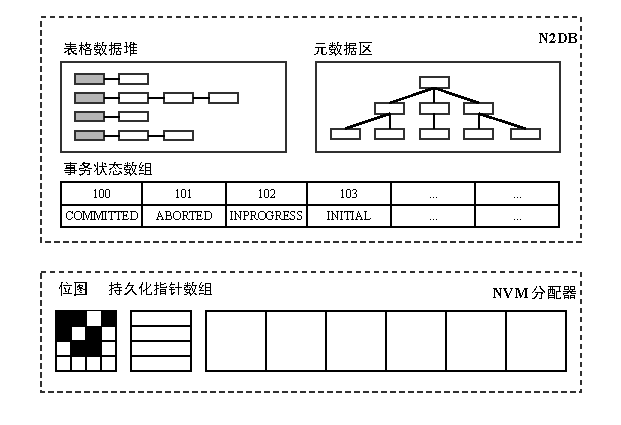
\includegraphics[width=1\linewidth]{figures/new-nvm-allocator}
    \caption{修改后的 N2DB 存储引擎的结构}
    \label{fig:nvm-allocator}
\end{figure}

\subsection{数据库元数据区的结构设计}

为了保证 N2DB 在故障恢复的过程中找到所有的数据库中所有的元数据, N2DB 需要增加一个元数据区负责存储和管理所有数据库的元信息。
元数据区的结构如图~\ref{fig:catalog} 所示。
元数据区中的数据结构组织成一颗三层高的树,其根节点的指针存储在 NVM 分配器的指针区域中。元数据区根据树的层次分别由三类数据结构,从根节点到叶节点分别是 N2DB 元数据,数据库元数据以及表格元数据。

\begin{figure}
    \centering
    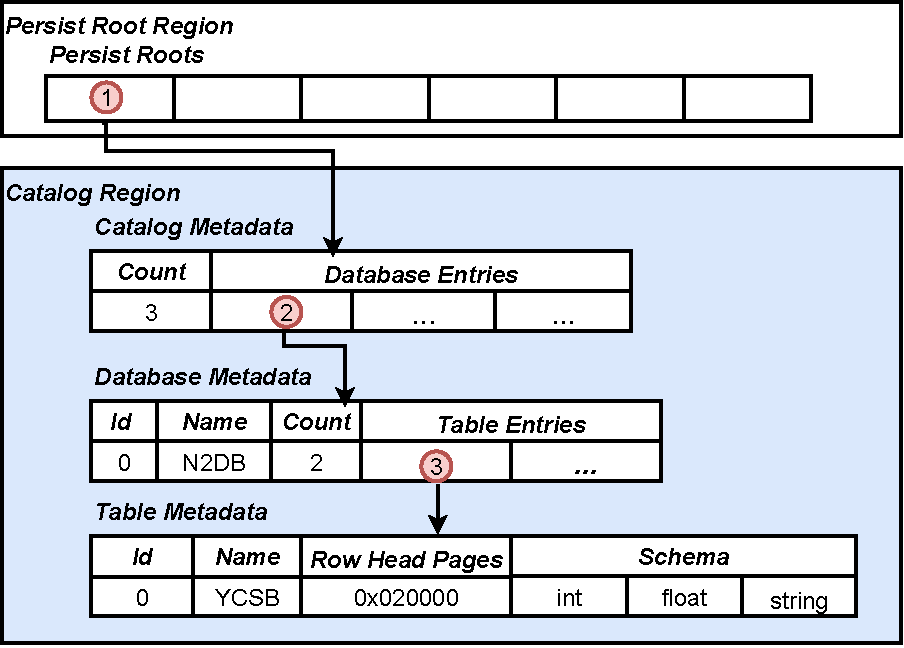
\includegraphics[width=1\linewidth]{figures/catalog.pdf}
    \caption{数据库元信息区的结构}
    \label{fig:catalog}
\end{figure}

N2DB 元数据中记录的整个存储引擎的元数据,比如存储引擎是否被初始化,这一轮的事务 ID 的起始值等信息。一个存储引擎可以创建多个数据库,因此 N2DB 元数据中还存放着数据库元数据的数量有以及各个数据库元数据的地址。

数据库元数据中存储这数据库的标识符,数据库的名称。同时数据库元数据中存储着一个定长的指针数组,其中的每个指针均是指向从属于该数据库的表格元数据。为了减少恢复时的开销,系统同样存储着表格数量。


表格元数据用于存储表格的所有元数据,包括表格的标识符等信息。同时表格元信息中也存储了模式信息,数据库管理系统可以借此计算出表格中所有的 head 和 version 的大小。在系统运行时,表格会将申请获得的页面的地址记录在表格元数据中。




\section{数据恢复机制设计思路}

根据上述三个设计目标,本文将 N2DB 的数据恢复流程分为三个阶段,分别是 NVM 分配器的恢复,数据库元数据的恢复以及记录数据的恢复。

\subsection{NVM 分配器的恢复}
\label{ssec:allocator-recovery}

NVM 分配器的恢复的目的在于回收所有未分配和分配但未被分配的页面。
当系统重启之后,N2DB 首先扫描 NVM 分配器的位图。
根据位图中的数据得到在系统宕机时的页面分配信息。
NVM 分配器将 bitmap 中所有状态为未分配的页面添加到一个空闲页面队列。

由于 NVM 分配器是无日志的分配的,因此位图中被标记位已分配的页面有可能没有任何数据结构使用该页面。
如果不回收此类页面则会造成内存泄漏。
然而根据 NVM 分配器自身的元数据无法回收分配但未被使用的页面。
此类页面会在后续步骤中由上层系统协助回收,具体的流程会在后续章节涉及到。

\subsection{数据库元数据的恢复}
\label{ssec:metadata-recovery}

数据库元数据的恢复的主要目的在于在 NVM 上找到所有数据库的数据结构,找到所有的记录相关的数据结构,重新设置数据库在重启之后的事务状态以及协助 NVM 分配器回收分配但未分配的空间。
数据库的元数据恢复的流程如下:

首先,N2DB 需要在 NVM 上找到所有元数据,并在内存中建立起数据库的索引。
目录是存储引擎中所有的数据库,表格以及列信息的索引。
N2DB 根据 NVM 分配器的接口得到 N2DB 元数据的地址。
由于 N2DB 上所有元数据组织成树状数据结构,N2DB 可以根据 N2DB 元数据中记录的信息,遍历地找到所有的数据库元数据以及表格元数据。
N2DB 在遍历树的过程中,需要根据持久化的元数据中的标记位信息来判断数据库或者表格是否创建成功。
如果数据库以及表格是创建失败的,N2DB 需要无视该数据库或表格的信息。
N2DB 将所有创建成功的数据库以及表格按照正确的层级关系添加到数据库目录中。
在此过程中,N2DB 需要统计所有创建成功的数据库和表格的元数据的空间使用情况。

其次,N2DB 根据表格的元数据中记录的 head 页面入口以及 version 页面入口得到所有表格的页面信息。
N2DB 根据表格元数据中的模式信息计算出各个表格的记录的 head 以及 version 的长度。
之后 N2DB 获得数据库中所有版本链的入口,以及表格中每个版本链所对应的行标识符。
在此过程中,N2DB 需要统计所有表格所管理的页面的使用情况。

接下来,N2DB 需要根据事务状态信息重新设置本轮运行的起始事务 ID。
事务状态数组中记录着上一轮活跃的事务 ID 的最大值以及最小值。
N2DB 根据事务状态数组中的数据更新本轮事务的起始 ID。
之后 N2DB 扫描事务状态数组中上一轮活跃的事务区间,将其中所有未结束的事务状态设置为 ABORTED。

最后,系统需要协助 NVM 分配器回收所有分配但未被使用的页面。
N2DB 在前几步记录了所有被数据库所使用的空间的信息。
之后 N2DB 将汇总后的空间使用情况传递给 NVM 分配器,NVM 分配器将会回收不被数据库使用的但状态为已分配的页面。



\subsection{记录数据的恢复}
\label{ssec:record-recovery}

当 N2DB 完成了数据库元数据的恢复阶段之后,N2DB 也得到了所有表格的记录相关的数据结构的信息。
系统接下来需要对于记录数据进行恢复,消除未提交事务所造成的片面影响。
如图~\ref{fig:record-recovery} 所示,记录数据的恢复流程可以分为三个阶段。

\begin{figure}[ht]
    \centering
    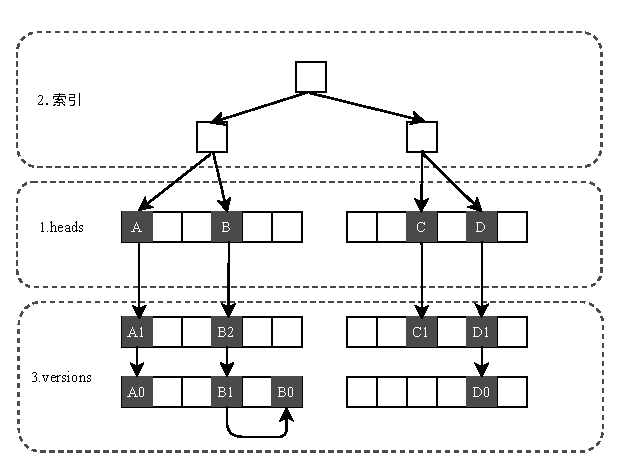
\includegraphics[width=1\linewidth]{recovery.pdf}
    \caption{记录数据的恢复步骤}
    \label{fig:record-recovery}
\end{figure}

首先是过滤所有不可见的以及未分配的 head。
一个数据库管理系统提供服务的前提是所有表格都有正确的索引来帮助事务查询,N2DB 也不例外。
N2DB 需要在所有可见的 head 上建立索引,因此需要将不可见的以及未分配的 head 过滤并回收掉。
表格的元数据中记录了 head pages,根据 head pages 中的地址,系统可以找到属于该表格的所有页面,进而找到了所有 head 的位置。
接下来系统需要扫描所有的 head,依次判断其是否是可回收的。
head 的可见性判断如图~\ref{fig:head-visibility} 所示。
head 首先需要判断最新版本是否为空,若为空则意味着该 head 是不可见的。
如果 head 对应的最新版本不为空,且最新版本是可见的,则意味着该 head 是可见的,因此该版本链是合法的。
版本可见性的判断与图~\ref{fig:version-visibility} 中相同。
最后如果 head 的最新版本是不可见的,但最新版本仍有较老的版本,那么该 head 也是可见的,版本链也是合法的。在此步骤中,由于 head 分配的无日志特性,系统只能通过扫描一个表格中所有的 head,依次判断每个 head 的可见性。同时系统在扫描的过程中会将所有不可见的版本回收,以防止内存泄漏问题。

\begin{figure}[ht]
    \centering
    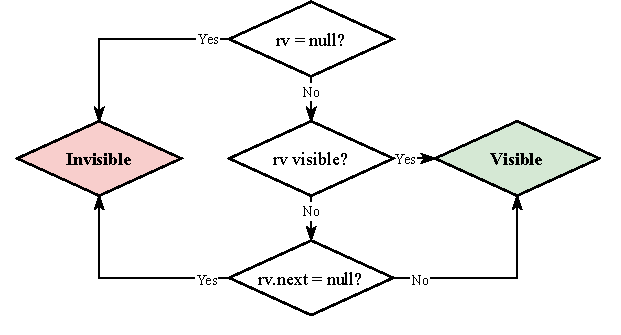
\includegraphics[width=1\linewidth]{figures/head_visibility.pdf}
    \caption{head 的可见性判断}
    \label{fig:head-visibility}
\end{figure}

第二是根据所有可见的 head 建立表格索引。
在扫描结束之后,系统将所有 head 对应的地址以及主键添加到新建的索引中。
版本链中此时仍存在不可见的版本,但是事务可以通过版本可见性无视版本链中中止事务以及中断事务所创建的不一致的 version。
因此当每个表格的索引重建之后,N2DB 就可以正常地相应请求了。

最后是回收所有未分配的 version。回收未分配的 version 是防止内存泄漏的关键。
由于 version 的分配也是无日志的,因此 version 分配与否当且仅当该 version 是否存在于一个合法的版本链中。
因此在索引建立之后,系统将会启动一个后台的扫描线程。
该线程负责扫描的版本链,并且记录版本链中所有 version 的位置信息。
该线程通过排除法可以得到所有未分配的 version 的位置信息,然后该线程会将未分配的 version 的信息传递给垃圾回收调度器。
后台扫描线程在扫描版本链的过程中,同样会识别出中止事务以及中断事务所创建的不可见的版本。
尽管这些版本不影响事务执行的正确性,但会影响事务的性能。因此后台扫描线程会将这些版本信息封装成 GCItem 传递给各个线程的垃圾回收调度器。

\section{数据恢复的正确性}

N2DB 中存在两个层面的数据管理。
一是 NVM 分配器采用页粒度管理和分配 NVM 空间。
二是 N2DB 中的表格在申请的页面上分配 head 以及 version。
因此 N2DB 需要保证两个层面的数据恢复工作都是正确的。

\subsection{NVM 分配器的数据恢复的正确性}

章节~\ref{ssec:nvm-alloc} 中定义了 NVM 分配器的可恢复性,即 NVM 分配器能否在重启之后将分配器的元数据中恢复到一个合法的状态。
合法的状态意味着对于 NVM 分配器而言,只有被使用的空间是已分配的,未被使用的空间均是未分配的,而且所有空间当且仅有一种状态。
一个空间被使用的判断标准在于该空间的地址是否被记录在 NVM 上。
根据 NVM 分配器的设计,一个页面在分配中,页面信息的记录一定晚于 bitmap 中分配信息的设置。
因此在系统重启之后,NVM 的页面当且仅有三种情况,未分配的,已分配且被使用的,以及分配但未被使用的。
前者可以通过章节~\ref{ssec:allocator-recovery} 中的步骤来回收,而第三种将由章节~\ref{ssec:metadata-recovery} 中的步骤来回收。
当两步回收均结束之后,NVM 分配器的元数据,也就是位图,会被设置成合法的状态。

\subsection{数据库的数据恢复的正确性}

数据库的数据恢复的正确在于能否保证提交事务的影响的持久化以及消除未提交事务的影响。

在元数据的恢复阶段中,N2DB 根据 NVM 分配器中的根指针,可以得到数据库中所有元数据的数据结构的地址信息。进而 N2DB 可以找到所有表格的记录相关数据结构的地址信息。

所有提交事务的影响包括 head 以及 version 的修改。由于系统保证在事务提交前事务的修改就已经持久化了,因此当 N2DB 找到所有版本链的入口时,提交事务的影响就没有丢失。未提交事务的影响同样也包括 head 以及 version 的修改。同时未提交事务包括两种,一种是中止事务,另一种是中断事务。

未提交事务对于 head 的影响是由 head 可见性来消除的。一个 head 是不可见的当且仅有三种情况:
\begin{enumerate}
    \item 该 head 是未分配的。一个 head 如果尚未被分配,那么该 head 的 newest\_version 应该为空指针。
    \item 该 head 是由一个中止事务或者中断事务插入的。根据章节~\ref{sec:mvcc} 中的插入流程,系统宕机可能发生在 head 修改 newest\_version 之前和之后。当宕机发生在 head 修改指针之前时,该 head 的 newest\_version 为空指针。当宕机发生在 head 修改指针之后时,该 head 的 newest\_version 所指向的版本应该是不合法的,其创建者也就是 xmin 对应的事务是未提交的。
    \item 该 head 已被删除,但尚未被垃圾回收。那么该 head 的 newest\_version 所对应的版本是被一个提交事务所废弃的。
\end{enumerate}
上述 head 的三种情况的分析可以看出 head 的可见性判断是完备的。
N2DB 根据 head 的可见性判断足以消除所有未提交事务对于 head 的影响。

未提交事务对于 version 的影响会被版本可见性判断无视掉。
一个未提交事务创建的版本当且仅有两种情况:
\begin{enumerate}
    \item 该 version 尚未被链接在版本链上。此类 version 会被后台的扫描线程视为未分配的,之后会被垃圾回收调度器回收。
    \item 该 version 已经被链接到版本链上,但事务未提交。version 的数据写入用于发生在其被链接在版本链上,因此 version 的 xmin 中的信息可以说明该版本是由一个未提交事务创建的。因此其他事务在运行时会无视掉此类版本。
\end{enumerate}
无论是哪一种情况,未提交事务相关的 version 都不会影响到后续事务的执行。

综上所述,N2DB 在数据恢复阶段结束后,提交事务的影响是持久化的。
而未提交事务的一部分影响被立刻消除。
另外一部分影响会被被其他事务无视,并且会被异步地消除。
因此 N2DB 的数据恢复机制是满足两个恢复原则的,其既可以保证事务的原子性也保证了事务的持久化。

\section{系统工程实现}
本章节将从代码级层面介绍数据恢复的机制的几个重要环节的系统工程实现。首先章节~\ref{ssec:data-structure-recovery} 会介绍 NVM 分配器的指针区域以及数据库的元数据的数据结构设计。
接下来章节~\ref{ssec:record-data-recovery} 会详细说明表格的记录数据恢复的流程。
最后章节~\ref{ssec:background-scan} 将简单提及后台扫描线程的流程。

\subsection{持久化指针的数据结构设计}
\label{ssec:data-structure-recovery}

为了保证系统能够在恢复时找到所有的数据结构,NVM 分配器中新增了持久化指针数组(PersistRootArray)这个数据结构。
持久化指针提供了访问指针以及持久化根指针的接口。
当系统第一次启动时会新建一个 N2DB 元数据,并且将根指针持久化到该数组第一个的位置。
持久化指针数组的数据结构定义如下:
\begin{itemize}
    \item 指针数量(root\_cnt):指针数量记录了存储于该数组的根指针的个数。
    \item 指针数组(roots):指针数组上记录了各个数据结构的根指针入口。
\end{itemize}



\subsection{元数据的数据结构设计}

数据库的所有元数据记录了存储引擎,数据库,表格以及列的所有元信息。
同时系统在创建数据库,表格等行为时,会修改不同类型的元数据。
为了保证数据结构的崩溃一致性,元数据的修改方法需要专门设计,以防止各个元数据之间数据的不一致。
本章节将依次介绍各个元数据的数据结构设计。

首先是 N2DB 的元数据。N2DB 的元数据主要记录着 N2DB 中数据库的数量以及各个数据库的元数据的指针。其具体的数据结构定义如下:
\begin{itemize}
    \item 初始化标志(is\_initialized):该标志表示该元数据是否被初始过。如果没有初始过则说明 N2DB 第一次启动。
    \item 数据库数量(database\_count):该变量记录了 N2DB 中数据库的数量。
    \item 数据库元数据入口(database\_entries):数据库元数据入口是一个数据库元数据指针的数组。
\end{itemize}

其次是数据库元数据。数据库元数据记录着数据库的标识符,名称等信息,同时存储着从属于该数据库的数量以及各个表格的元数据的指针。
具体的数据结构定义如下:
\begin{itemize}
    \item 初始化标志(is\_initialized):该标志用于判断该元数据是否被初始过。数据库在创建的过程中会先设置其他的成员变量的数据,最后原子化设置该标志,如果该标志不为 1,则数据库视为创建失败。
    \item 数据库标识符(database\_id):每个数据库都有全局唯一的数字标识符。
    \item 表格数量(table\_count):该变量记录了从属于数据库的表格的数量。
    \item 表格元数据入口(table\_entries):表格元数据入口是一个定长的数组,其中每一个元素均是表格元数据的指针。。
\end{itemize}

最后是表格元数据。
表格元数据记录着表格标识符,名称等基本信息。
表格元数据还记录着表格的模式信息,即每个列的类型,大小,名称等信息。
由于表格会在运行时申请页面,表格元数据中还需要记录表格申请的页面的地址。
表格元数据的数据结构定义如下:
\begin{itemize}
    \item 初始化标志(is\_initialized):该标志用于判断该元数据是否被初始过。
    \item 表格标识符(table\_id):每个表格的全局唯一的数字标识符。
    \item 列数(col\_count):列数记录了表格的列的数量。
    \item 列信息数组(col\_infos):列信息数组用于记录表格的模式信息。数组中每一个列信息均是一个三元组,分别记录了列名称,列大小以及列类型。
    \item head 页面入口(head\_pages\_entris):head 页面入口是一个数组,其中每一个元素均是一个页面指针。每个页面都是专门用来存放表格的 head。
    \item version 页面入口(version\_pages\_entries):version 页面入口同样也是一个页面指针数组。其中的每个页面都是专门用来存放表格的 version。
\end{itemize}


\begin{algorithm}[ht]
    \caption{使用表格名称创建一个新的表格, $create\_table\_with\_name$}
    \label{alg:create-table}
    \KwIn{The name of new table, $tbl\_name$ and schema}
    \KwOut{Success or not}
    \BlankLine
    Lock the database metadata;

    \If{ A table named $db\_name$ found}{
        Unlock the database metadata;

        return $false$;
    }

    NVM allocator a new page, $table\_data$;

    Get a new table id, $table\_id$;

    NVM allocator two new page for a new table;

    Modify $table\_data$ and persist;

    $table\_entries[table\_count] = table\_data$;

    Fence;

    $table\_count++$;

    Fence;

    Unlock the database metadata;

    return $true$;
\end{algorithm}

如前文所说,N2DB 中的数据库的创建,表格的创建会涉及多个元数据。
以创建表格为例,N2DB 在创建表格的过程会修改分配器的元数据,数据库的元数据以及表格的元数据。
如何正确设计几个元数据之间的持久化顺序是一大问题。
本文所实现的创建表格的具体流程展示在算法~\ref{alg:create-table} 中。
首先数据库元数据需要上锁,以防止别的线程并发访问该元数据。
接下来 NVM 分配器分配一个新的页面给表格元数据。
数据库元数据获取一个新的表格标识符。
NVM 分配器为表格多申请两个页面。表格需要这两个页面存放页面指针。
之后表格相关的元数据,比如表格标识符,名称,模式信息以及两个页面指针数组的地址都记录在 $table\_data$ 中。
之后系统更新数据库元数据,并且解锁该元数据。

通过该流程可以看出,如果系统在中间的步骤宕机了,会导致各个元数据之间的数据的不一致。
在数据恢复阶段,系统仅根据表格数量就来判断表格创建与否,而不根据其他信息。
根据创建表格这个例子可以看出,即使创建表格的过程中写的数据量远大于一个字节,系统仍可以通过一个字节的原子写来保证此过程的原子性。数据库中其他元数据的更新流程也是遵循此原则设计的。
不过该设计方法会在恢复时引入一些额外的开销。如果在数据恢复阶段系统发现了元数据之间的不一致,系统需要立刻对元数据进行修改。


\subsection{表格记录数据的恢复流程}
\label{ssec:record-data-recovery}

\begin{algorithm}[ht]
    \caption{表格重新加载 head 的流程,$reload\_head$}
    \label{alg:reload-heads}
    \BlankLine

    Calculate the length of head;

    Calculate the number of head in one page, $head\_per\_page$;

    Create a new index;

    \For{
        page $p$ in $head\_page\_entries[0:head\_page\_count]$
    }
    {
        \For{
            head $rh$ in $p[0:head\_per\_pages]$
        }{
            $rv = rh.newset\_version$;

            \eIf{$is\_recyable(rh)$}{
                Table reclaims $rh$;
            } {
                Insert $rh$ in the index;
            }

        }
    }
\end{algorithm}



N2DB 的过滤不可见的 head 流程如算法~\ref{alg:reload-heads} 所示。
系统根据元数据中的模式信息计算出一个 head 的长度以及一个页面上能够存放几个 head。
接下来系统创建一个新的索引。
系统根据 $head\_page\_entries$ 以及 $ head\_page\_count$ 两个数据得到该表格用于存储 head 的所有页面的地址。系统扫描每个页面上的所有的 head,依次判断各个 head 是否满足回收条件,并且回收可回收的 head。

\begin{algorithm}[ht]
    \caption{判断 head 是否可以回收,$is\_recyclable$}
    \label{alg:head-visibility}
    \KwIn{A head, $h$}
    \KwOut{Recyclable or not}
    \BlankLine

    $v = h.newest\_version$

    \If{$v == nullptr$}{
        return $true$;
    }


    \If{The transaction with $rv.xmax$ is COMMITTED} {
        return $true$;
    }

    \If{The transaction with $rv.xmin$ is ABORTED and $rv.prev\_version == nullptr$} {
        return $true$;
    }

    return $false$;


\end{algorithm}

算法~\ref{alg:head-visibility} 中展示了判断 head 是否可回收的具体过程。
首先查看该 head 的最新版本,若为空则该 head 可回收。
然后判断最新版本是否是提交事务删除的,如果是的话,则该 head 可回收。
最后判断最新版本的创建是否为中止的,并且没有更老的版本,如果满足该条件则该 head 也是可回收的。

\subsection{后台扫描线程的设计}
\label{ssec:background-scan}

后台扫描线程会依次回收每个表格的未分配的空间。后台线程扫描一个表格的版本链的过程如算法~\ref{alg:scan-versions} 中所示。扫描函数的输入分别是一个表格的可见的 head 的集合以及在系统重启时该表格的 $version\_page\_count$。$sacn\_version\_chain$ 函数首先创建两个数组,一个用于存储 version 的地址,一个用于存储扫描过程中遇到的不可见的 version。
接下来该线程将扫描所有的版本链,并且记录所有 version 的地址,如果该 version 是不可见的,将其封装成一个 GCItem。该线程会将一部分的 version 过滤掉。这部分 version 不属于该表格在数据恢复时的 $version\_page\_entries$ 的页面。线程将剩余的 version 排序,并且生成未分配的 version 的数组。
最后线程依次回收的 version,并且将扫描过程中遇到的不可见的 version 所对应的 GCItem 传递给垃圾回收调度器。


\begin{algorithm}[ht]
    \caption{数据恢复阶段的后台的扫描流程,$scan\_version\_chain$}
    \label{alg:scan-versions}
    \KwIn{Visible heads of a table, $heads$, $version\_page\_count$}
    \BlankLine

    Create a empty array of version, $versions$

    Create a empty array of GCItem, $gc\_list$

    \For{ head $h$ in $heads$}{
        \For{
            version $v$ in the version chain of $h$
        }{
            Insert $v$ into $versions$;

            \If{
                $v$ is invisible
            }{
                Pack $v$ as a GCItem and insert it into $gc\_list$;
            }
        }
    }

    Filter out $v$ that is not in $version\_page\_entries[0:version\_page_count]$;

    Sort $versions$ according to address;


    Generate unallocated versions $unallocated\_versions$ using $versions$;

    \For{version $v$ in $unallocated\_version$}{
        Table reclaims $v$;
    }

    \For{
        GCItem $item$ in $gc\_list$
    }{
        GCScheduler.schedule(item);
    }

\end{algorithm}

\section{本章小结}

本章节主要介绍了数据恢复机制的设计目标,设计思路以及正确性,其中还介绍了存储引擎的修改。同时为了详细介绍数据恢复的流程,本章节还从代码层面介绍了数据恢复机制中相关的三个重要的环节。

首先是数据恢复机制的设计目标。
虽然 NVM 的数据是持久化的,但是如果没有正确的元信息,NVM 上的数据将无法解读的字节流。
因此 N2DB 需要能够找到 NVM 上所有的数据结构。同时又因为 N2DB 需要保证事务的持久化以及原子性,数据恢复机制还对记录数据进行恢复。本文将设计目标总结为三点,分别是重构页面分配信息,恢复数据结构以及保证事务的原子性和持久化。

接着是存储引擎的修改。为了达成三个设计目标,N2DB 必须修改存储引擎的结构,尤其是 NVM 分配器和元数据的存储方式。NVM 分配器中添加一个持久化指针数组,其用于存储所有数据结构的根指针。
而存储引擎新增了元数据区,以树状结构来组织和管理各个层级的元数据。

然后是数据恢复机制的设计思路。
根据三个设计目标,本文将数据恢复流程大致分为三个阶段。
首先是 NVM 分配器的恢复。NVM 分配器是负责管理和分配 NVM 空间的。
因此 NVM 分配器的页面分配信息必须恢复到合法的状态,NVM 分配器还需要回收未分配及分配但未被使用的的页面。
接下来是元数据的恢复,本文将元数据组织成一个树状结构,并且在各个层级都存储了重要的元信息。
因此系统在数据恢复的过程中能够找到所有数据结构的位置。
系统同样需要根据元信息正确设置事务相关的状态,同时协助 NVM 分配器回收分配但未被使用的空间。最后则是记录数据的恢复,记录数据的恢复的目的在于遵循两个恢复原则,重新构造索引以及回收未分配的空间。记录数据恢复分为三步,过滤不可见的 head,重新构造索引以及使用后台扫描线程回收未分配的 version。系统重新构造索引后就能正常地提供服务。

之后是数据恢复机制的正确性。N2DB 的数据恢复的正确性可以分为两个层面。一层面是 NVM 分配器的数据恢复的正确性,这取决于在恢复后,NVM 分配器能否得到正确的分配信息。
另一部分是数据库的数据恢复的正确性,这取决于两点,一个保证提交事务的影响的持久化,二是消除未提交事务的影响。通过对每种情况分类讨论,本章节论证了 N2DB 数据恢复机制的正确性。

最后是数据恢复机制的系统实现。本章节首先介绍了持久化数组以及各个元数据的数据结构设计。
本章节进一步阐述了所有 NVM 数据结构修改的原则,即通过原子修改一个标志位来原子化一个复杂的数据结构修改。
接着本章节介绍了数据恢复过程中较为重要的记录数据恢复的流程,同时从代码层面解释 head 可见性的判断标准。
最后本章节介绍了后台扫描线程的主要工作流程。



% !TeX root = ../thuthesis-caishiyu.tex

\chapter{实验与评价}

本章节主要介绍 N2DB 的垃圾回收机制以及数据恢复机制的实验与评价。
本文使用 TPC-C 以及 YCSB 两种实验负载对 N2DB 以及 InnoDB 进行实验,主要的测试目标为:
\begin{itemize}
    \item N2DB 在开启和关闭垃圾回收机制下系统的运行性能对比以及存储空间使用量对比
    \item N2DB 和 MySQL 在相同条件下数据恢复的时间对比以及存储空间使用量对比
\end{itemize}

本章节首先介绍实验的环境设置,包括实验环境的硬件条件,NVM 的工作模式以及两个系统的参数设置。接着本章节介绍使用的两个负载的基本情况以及参数设置。之后的章节将会从垃圾回收以及数据恢复两个方面进行实验,并对实验数据进行分析。

\section{实验设置}

本文的实验均在同一台服务器上运行。该服务器有 4 个 Intel Xeon Gold 5220 处理器。每个处理器上有 18 个核。
Intel Optane DC PMM 是安装在处理器的内存插槽的。一个处理器有 6 个内存插槽,Intel Optane DC PMM 的容量是 128 GB,因此一个处理器的 NVM 空间至多为 768 GB。由于非统一内存访问(NUMA)效应,线程跨核访问 NVM 空间的性能会显著下降。因此本文的实验均在同一个核上进行。本实验中 NVM 的使用模式有 DAX 模式以及文件系统模式,两种模式的性能差异如表格~\ref{tab:nvm-metric} 所示。

\begin{table}
    \centering
    \caption{NVM 文件系统模式以及 DAX 的模式的访问性能对比}
    \begin{tabular}{lll}
        \toprule
        指标           & 文件系统模式 & DAX 模式 \\
        \midrule
        读带宽(GB/s) & 4.7          & 23       \\
        写带宽(GB/s) & 1.8          & 11       \\
        读延迟(ns)   & 1700         & 310      \\
        写延迟(ns)   & 5500         & 105      \\
        \bottomrule
    \end{tabular}
    \label{tab:nvm-metric}
\end{table}

本文用于对比的系统是 InnoDB。InnoDB 是 MySQL 的存储引擎,其接口与 N2DB 十分相近。
在本实验中,InnoDB 使用文件系统模式使用 NVM 空间。
InnoDB 使用 WAL 来记录事务的操作,同时使用 ARIES 算法来进行数据恢复。
$log\_file\_size$ 是 InnoDB 的一个影响恢复性能的重要参数,其含义为 InnoDB 的日志文件大小。
通常 InnoDB 的日志数量为两个,InnoDB 会交替使用两个日志。当一个日志写满时,InnoDB 会进行一次 checkpoint 操作,之后切换到另外一个日志。因此 $log\_file\_size$ 影响 InnoDB 的运行时性能以及恢复时的性能。当 $log\_file\_size$ 越大时,InnoDB 生产 checkpoint 的频率越低,系统运行时的性能提高。但是 checkpoint 的频率降低意味着 InnoDB 在重启之后需要处理的日志的数量增多,因此会增加恢复时间,同时也会增大存储空间的使用量。在本文中,$log\_file\_size$ 被设置为 64 MB,128 MB 以及 256 MB。
InnoDB 使用文件系统模式访问和管理 NVM。

N2DB 在本实验中使用 $gc\_threshold$ 参数来控制垃圾回收的频率。在垃圾回收的对比实验中,gc\_threshold 被设置为 100。

\section{实验负载}

本实验使用 YCSB 以及 TPC-C 两种实验负载来测试 N2DB 的垃圾回收机制和数据恢复机制的性能。

YCSB 是雅虎公司对云服务进行性能测试的工具。YCSB 主要测试的事务操作是读,更新以及范围查询。
YCSB 的测试数据库中仅有一个张表格。表格中一共有 10 列,其中包含一个主键以及 9 个字节类型的列。每列的长度为 10 字节,因此一条记录为 100 字节。本实验中 YCSB 的测试表格中一共有 1000000 条记录。表格的数据大小在 1 GB 左右。
YCSB 中的每个事务会进行 10 次操作,每次操作的类型是随机的。本实验中所使用 YCSB 根据操作类型的分布可以分为三类,分别是:
\begin{enumerate}
    \item \textbf{读偏向型:}$90\%$ 读操作,$10\%$ 写操作;
    \item \textbf{平衡型:}$50\%$ 读操作,$50\%$ 写操作;
    \item \textbf{写偏向型:}$10\%$ 读操作,$90\%$ 写操作;
\end{enumerate}


TPC-C 是针对联机交易类型(OLTP)数据库设计的性能测试工具。TPC-C 模拟了一个电商环境。在该环境中,用户可以发布新的交易订单,供应商会根据仓库以及辖区的存储信息进行货物配送以及资金结算。
TPC-C 的测试数据库一共包含 9 张表,包括仓库,用户,订单等。TPC-C 测试中,事务会按照一定分布执行 5 个类型的操作。在本文的实验设置中,仓库数量固定为 8 个,并且所有表格数据初始大小控制在 1 GB 左右。

\section{垃圾回收性能对比实验}

本章节将比较开启与关闭垃圾回收机制对于系统运行时性能以及存储空间的影响。本章节将使用三种类型的 YCSB 以及 TPC-C 进行实验。

\begin{figure}
    \centering
    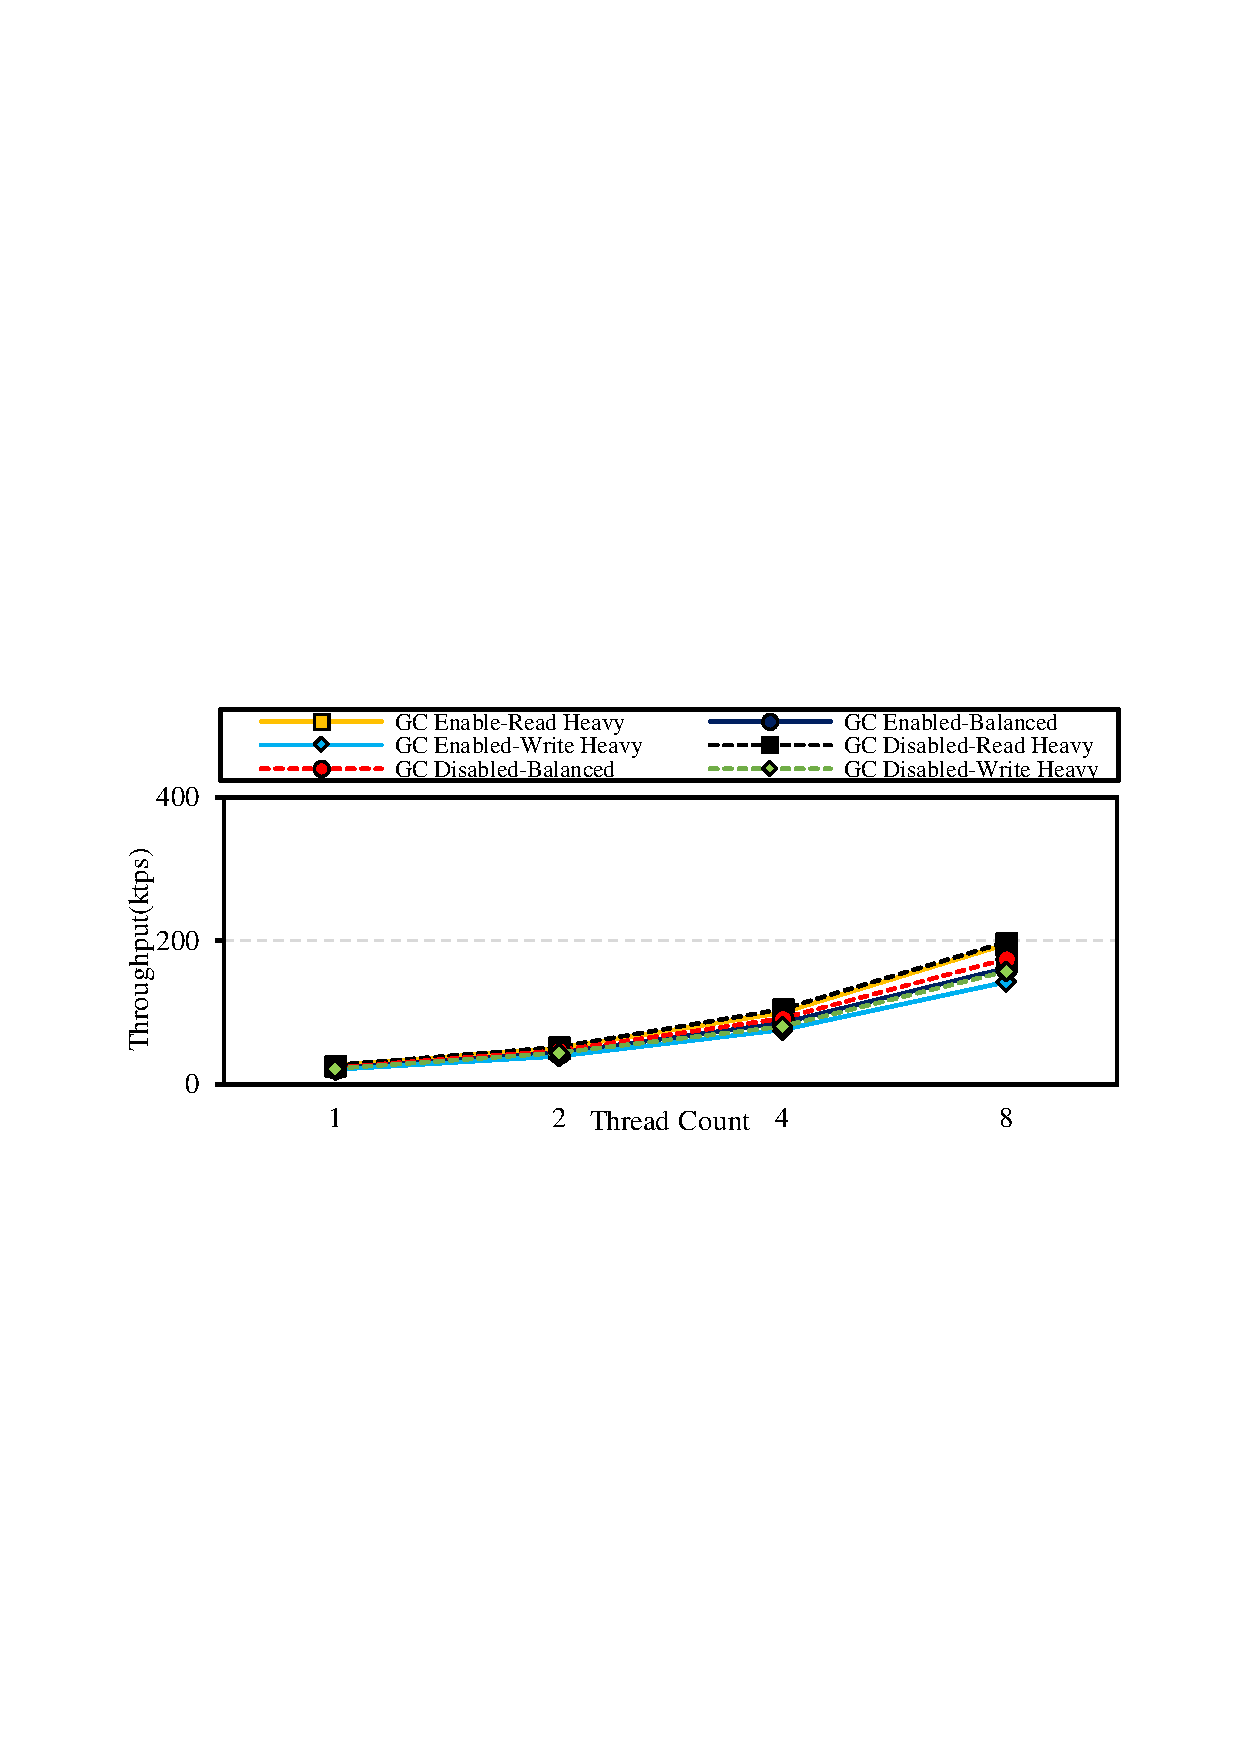
\includegraphics[width=15cm, trim={1cm 9cm 1cm 10cm}]{figures/gc-ycsb-throughput.pdf}
    \caption{YCSB 负载下垃圾回收性能的吞吐率对比实验}
    \label{fig:gc-throughput-ycsb}
\end{figure}

\subsection{运行时性能对比}

首先是三种 YCSB 负载下的运行时性能对比。如图~\ref{fig:gc-throughput-ycsb} 所示,整体上开启垃圾回收比关闭垃圾回收的运行时性能至多慢 $10\%$。在读偏向型的 YCSB 负载下,开启垃圾回收的系统性能比关闭垃圾回收的系统少 $2\%$ 左右。这是因为读偏向型负载下,事务更新数量少,因此产生的不可见版本少,没有垃圾回收的必要,而且垃圾回收机制本身引入了额外的开销。平衡型的实验结果也与读偏向型负载相似,开启垃圾回收的系统的吞吐率相对于关闭的系统少约 $7\%$。写偏向型的实验结果中,单核时开启的系统相对于关闭的系统少 $7\%$。随着核数增多,这个差异增大到 $10\%$。这是因为引入垃圾回收会增大线程之间冲突的概率,额外的锁开销也会影响运行时的事务的性能。因此二者的差异会随着核数的增加而增加。


\begin{figure}
    \centering
    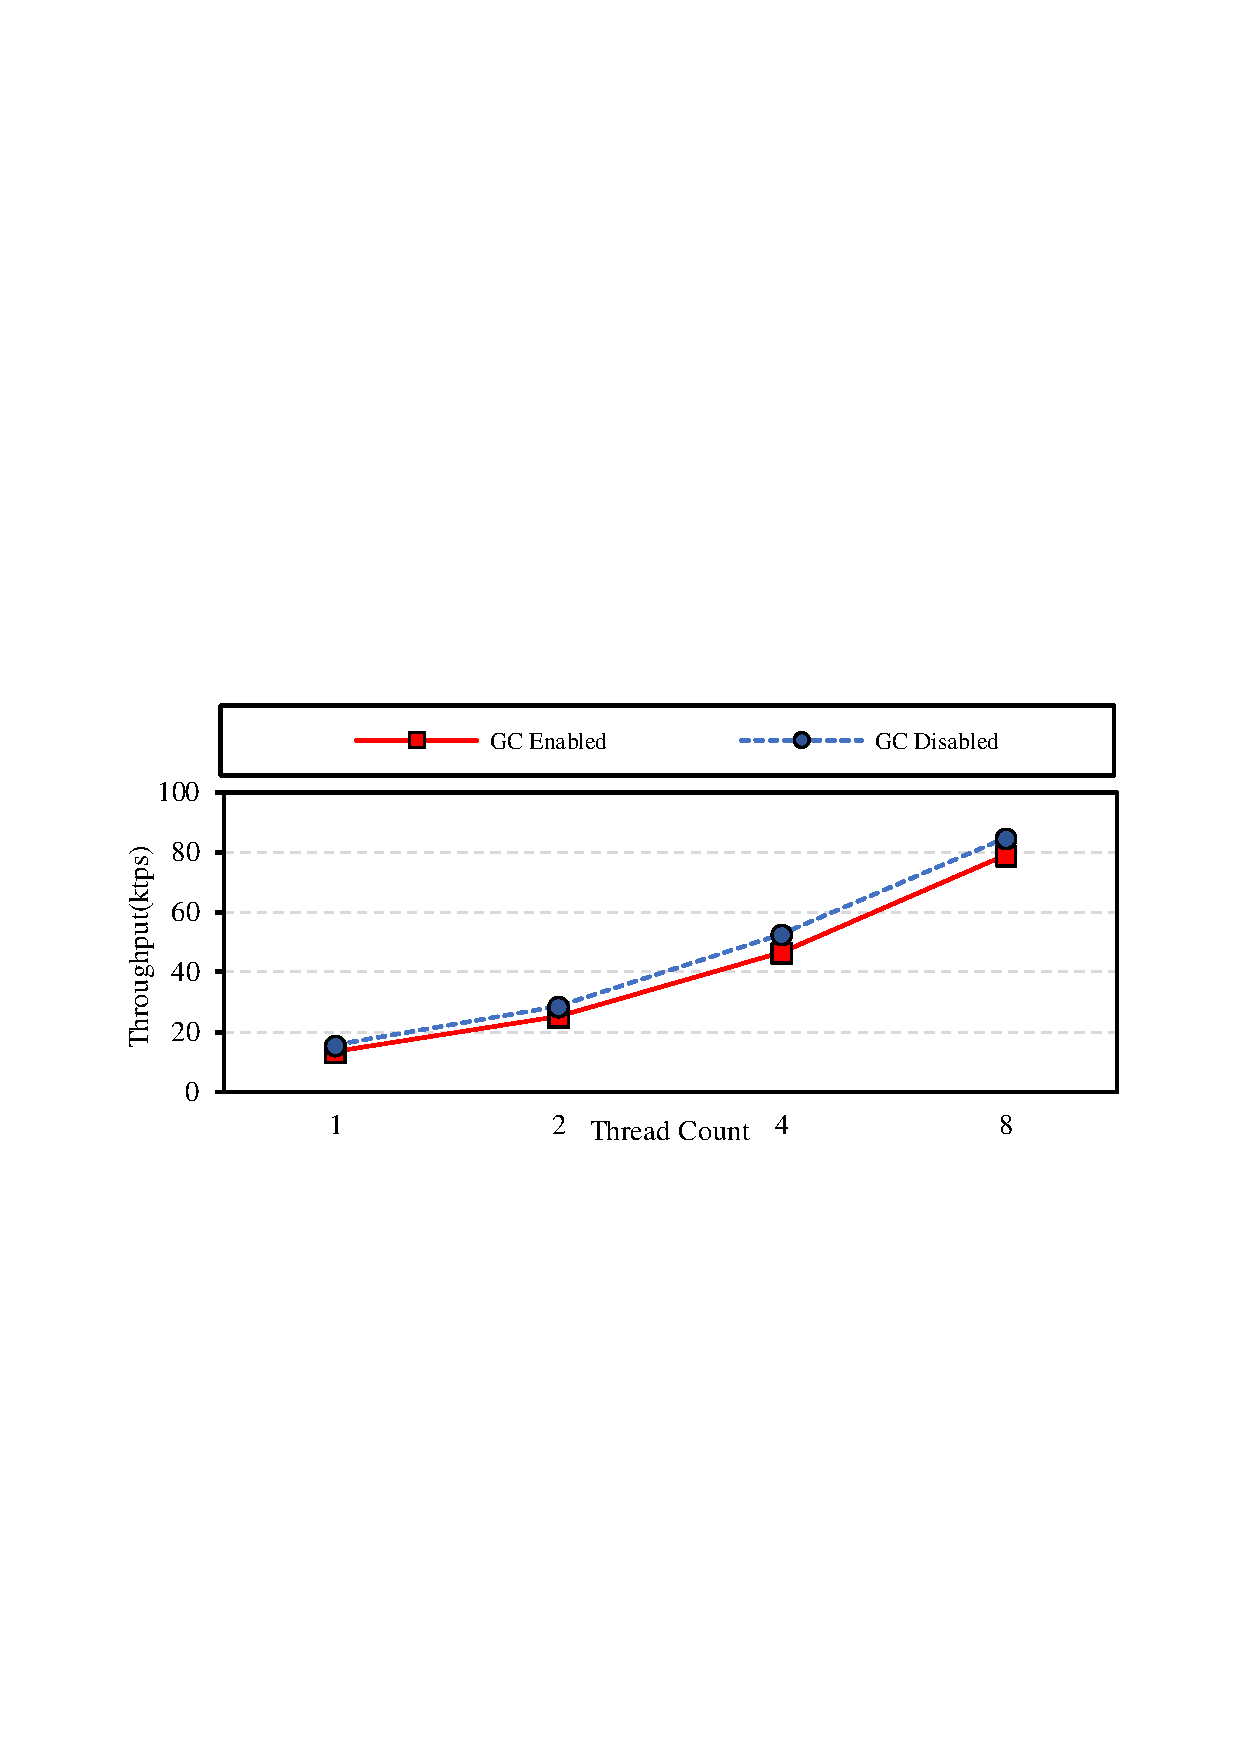
\includegraphics[width=15cm, trim={1cm 9cm 1cm 10cm}]{figures/gc-tpcc-throughput.pdf}
    \caption{TPC-C 负载下垃圾回收性能的吞吐率对比实验}
    \label{fig:gc-throughput-tpcc}
\end{figure}

接下来是 TPC-C 负载下的运行时性能对比。如图~\ref{fig:gc-throughput-tpcc} 所示,TPC-C 负载下的性能差异与写偏向型的 YCSB 负载下的性能差异相近。这是因为 TPC-C 负载中,事务的操作类型大多是更新操作。



\subsection{存储空间对比}

三种 YCSB 以及 TPC-C 负载下的存储空间对比如图~\ref{fig:gc-storage-ycsb} 以及图~\ref{fig:gc-storage-tpcc} 所示。
在读偏向型的 YCSB 负载的实验结果中,开启垃圾机制至多节省 $20\%$ 左右的存储空间。
随着负载中的更新事务的占比的提高,垃圾回收所节省的存储空间的比例也逐渐上升。
平衡型 YCSB 负载中垃圾回收至多节约了 $55\%$,而在写偏向型负载和 TPC-C 负载中,对应的比例分别为 $67\%$ 和 $50\%$。

\begin{figure}
    \centering
    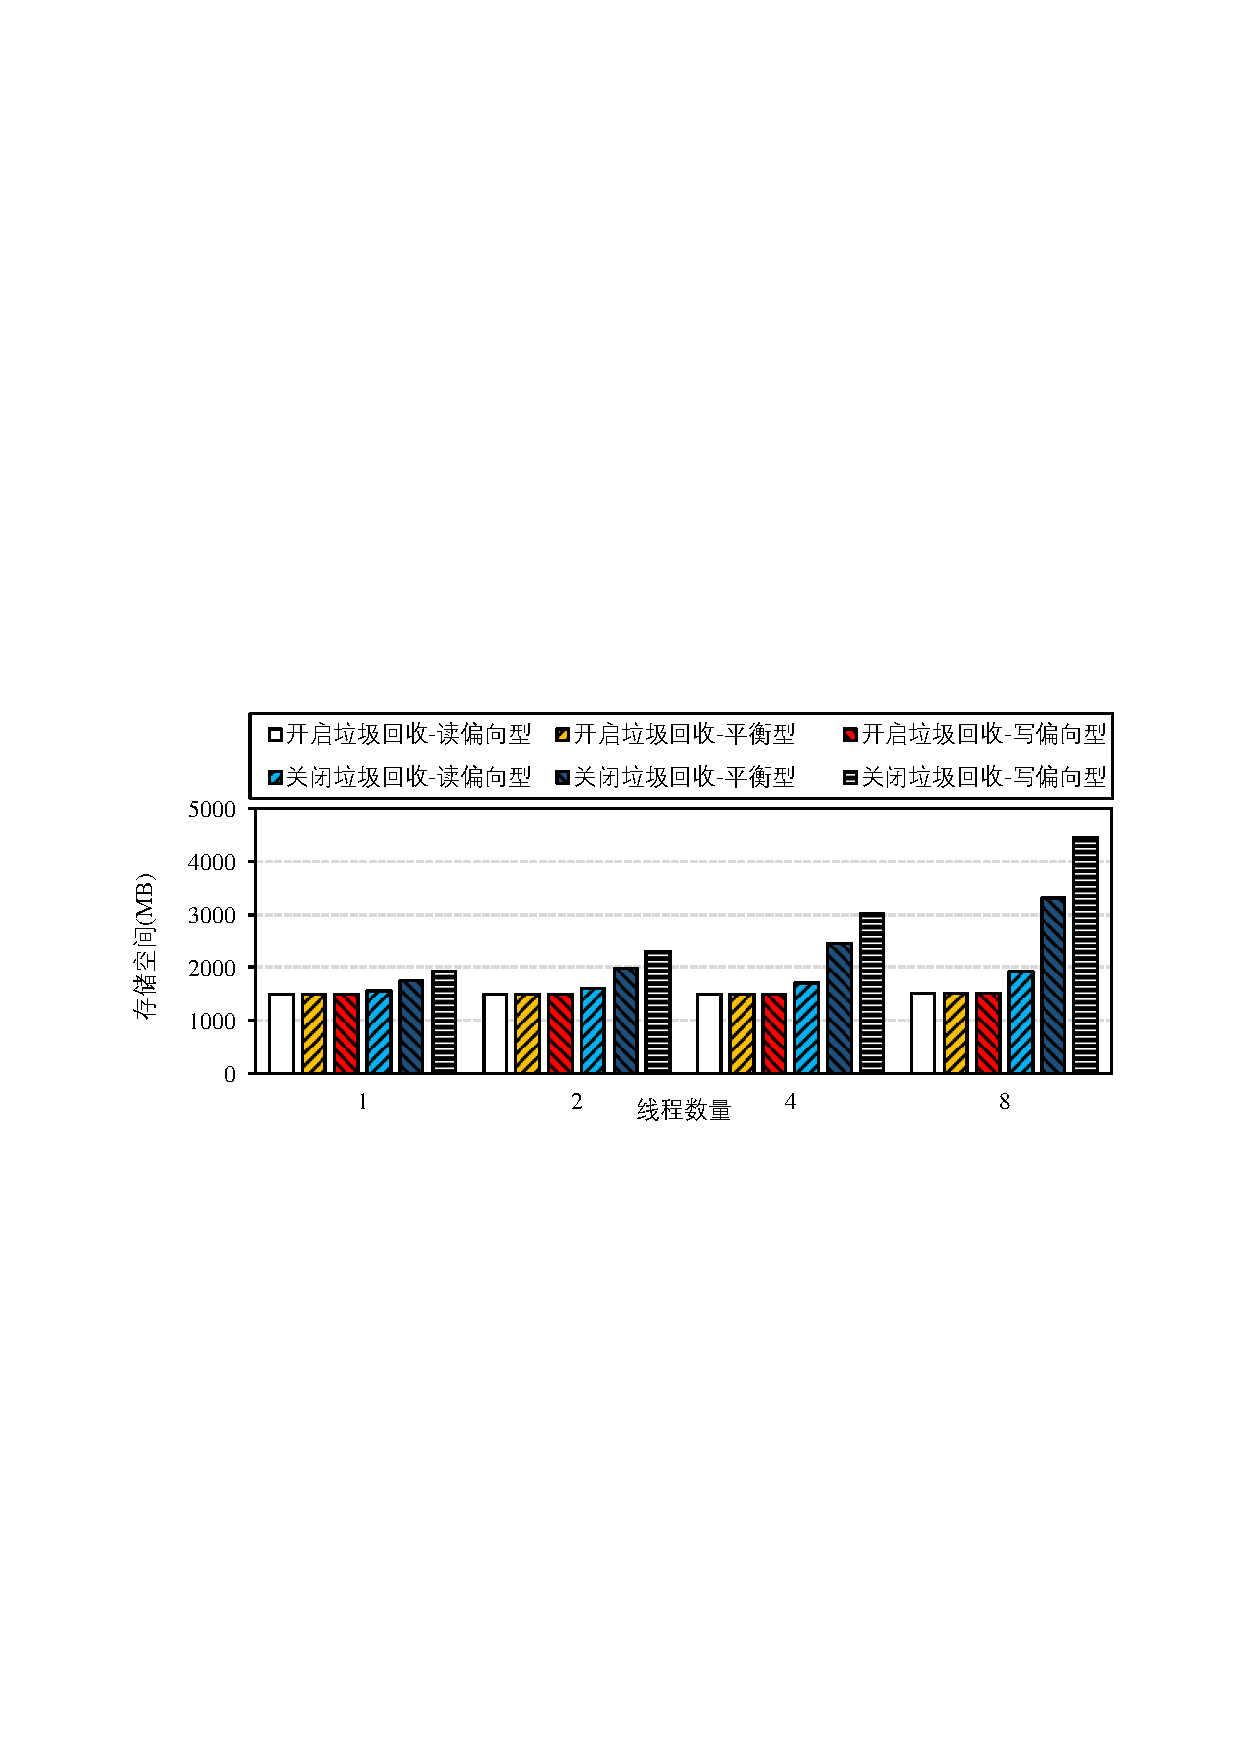
\includegraphics[width=15cm, trim={1cm 9cm 1cm 10cm}]{figures/gc-ycsb-storage.pdf}
    \caption{YCSB 负载下垃圾回收性能的存储空间对比实验}
    \label{fig:gc-storage-ycsb}
\end{figure}

\begin{figure}
    \centering
    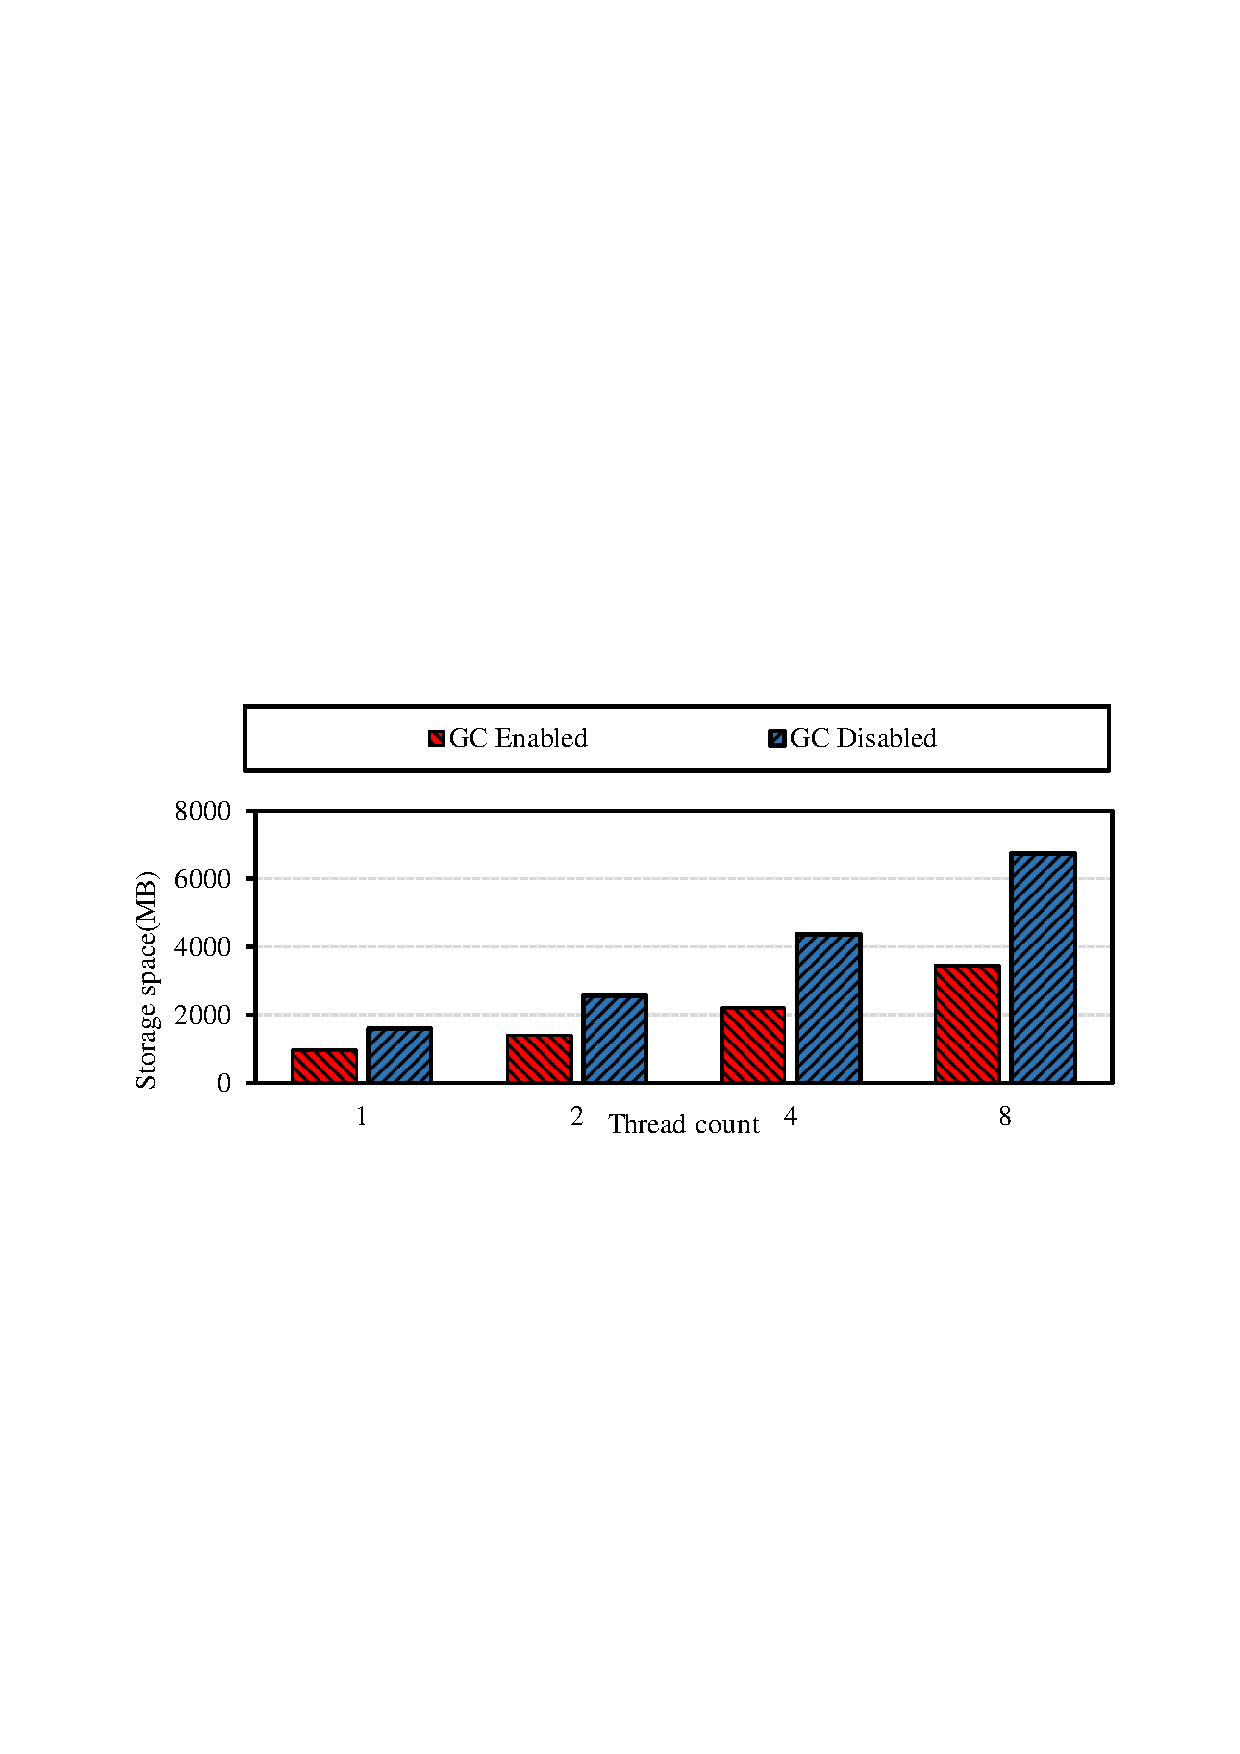
\includegraphics[width=15cm, trim={1cm 9cm 1cm 10cm}]{figures/gc-tpcc-storage.pdf}
    \caption{TPC-C 负载下垃圾回收性能的存储空间对比实验}
    \label{fig:gc-storage-tpcc}
\end{figure}

整体上而言,垃圾回收机制对于 N2DB 此类基于多版本并发控制的算法的系统效果显著。
并且效果随着系统中的更新操作的所占的比重增加而增加。


\section{数据恢复性能对比实验}

本章节将对比 N2DB 与 InnoDB 的数据恢复性能。两个系统均使用平衡型的 YCSB 负载。
当事务提交的数量达到一个阈值时,测试工具将使用 SIGKILL 强制结束两个系统,之后记录两个系统的恢复时间以及存储空间使用情况。在本实验中,实验使用不同提交事务的阈值来进一步对比恢复性能差异。在本实验设置中,提交事务的阈值分别是 10000 和 100000。

\subsection{数据恢复时间对比}

首先是在数据恢复的时间对比。实验结果如图~\ref{fig:recovery-time-analysis} 所示。
总体上而言,N2DB 的恢复时间远小于 InnoDB 的恢复时间。前者大约比后者小三个数量级。
造成这一差异的主要原因在于基于 WAL 的恢复机制的复杂性。
该机制要求系统在数据恢复时扫描日志,分析系统中断的状态。
之后系统需要重做检查之后的所有日志来将系统的状态恢复到系统故障的时刻的状态。
最后在回滚阶段,系统需要回滚所有未提交事务的操作。
并且该机制要求系统只有在回滚操作全部结束后才能相应服务。
N2DB 从并发控制算法的角度保证了提交事务的影响的持久化,因此在数据恢复时不需要重做。
对于 N2DB 中的中止事务的影响,对于 head 的影响会被立刻回收,而对于 version 的影响会根据可见性判断无视掉。
N2DB 仅需要得到索引重建之后就能提供服务。

从 InnoDB 的实验结果可以看出,不同的 $log\_file\_size$ 会显著影响恢复时间。
在本文的实验中,256 MB 相对于 64 MB 仅能带来 $10\%$ 的性能提升,同时会导致恢复时间提高 $70\%$。


\begin{figure}
    \centering
    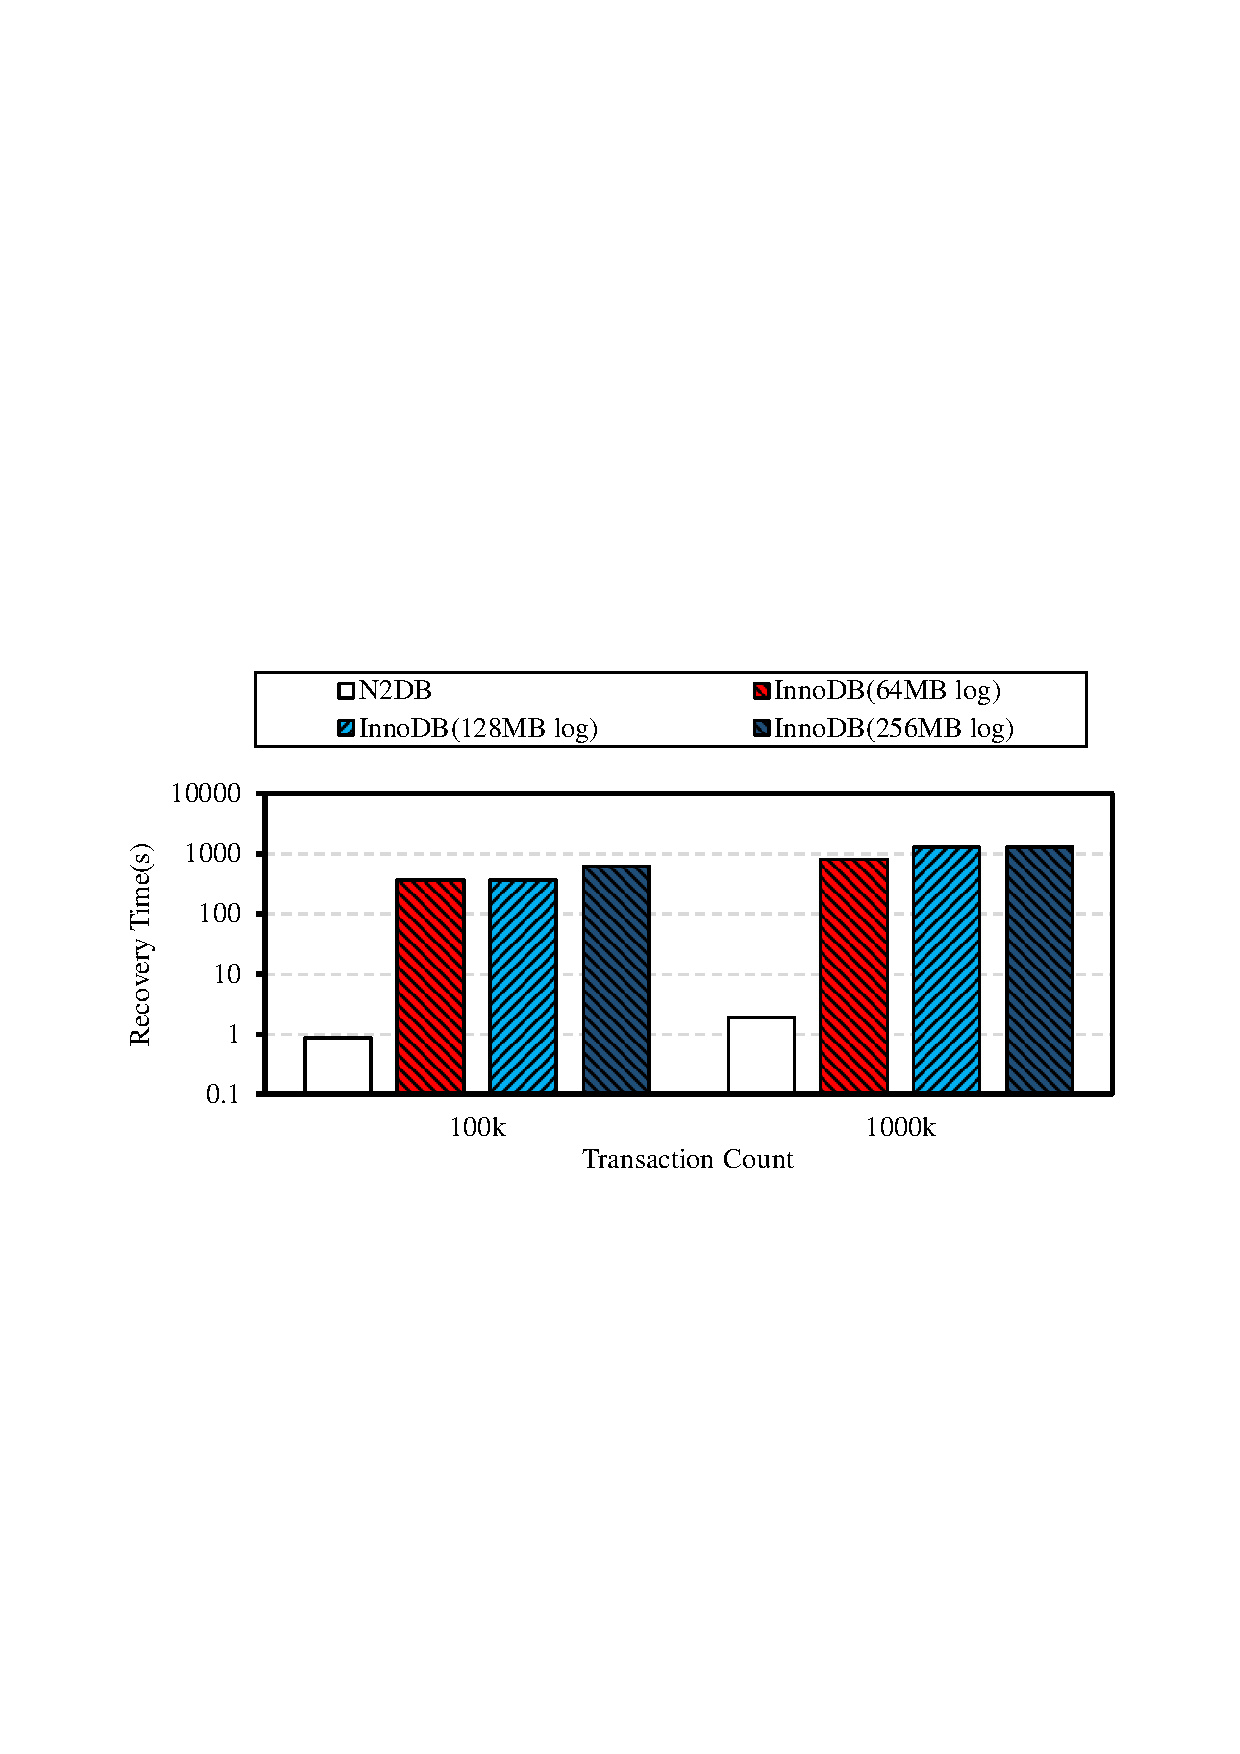
\includegraphics[width=15cm, trim={1cm 9cm 1cm 10cm}]{figures/recovery-time.pdf}
    \caption{YCSB 负载下数据恢复的时间对比实验}
    \label{fig:recovery-time-ycsb}
\end{figure}

\begin{figure}
    \centering
    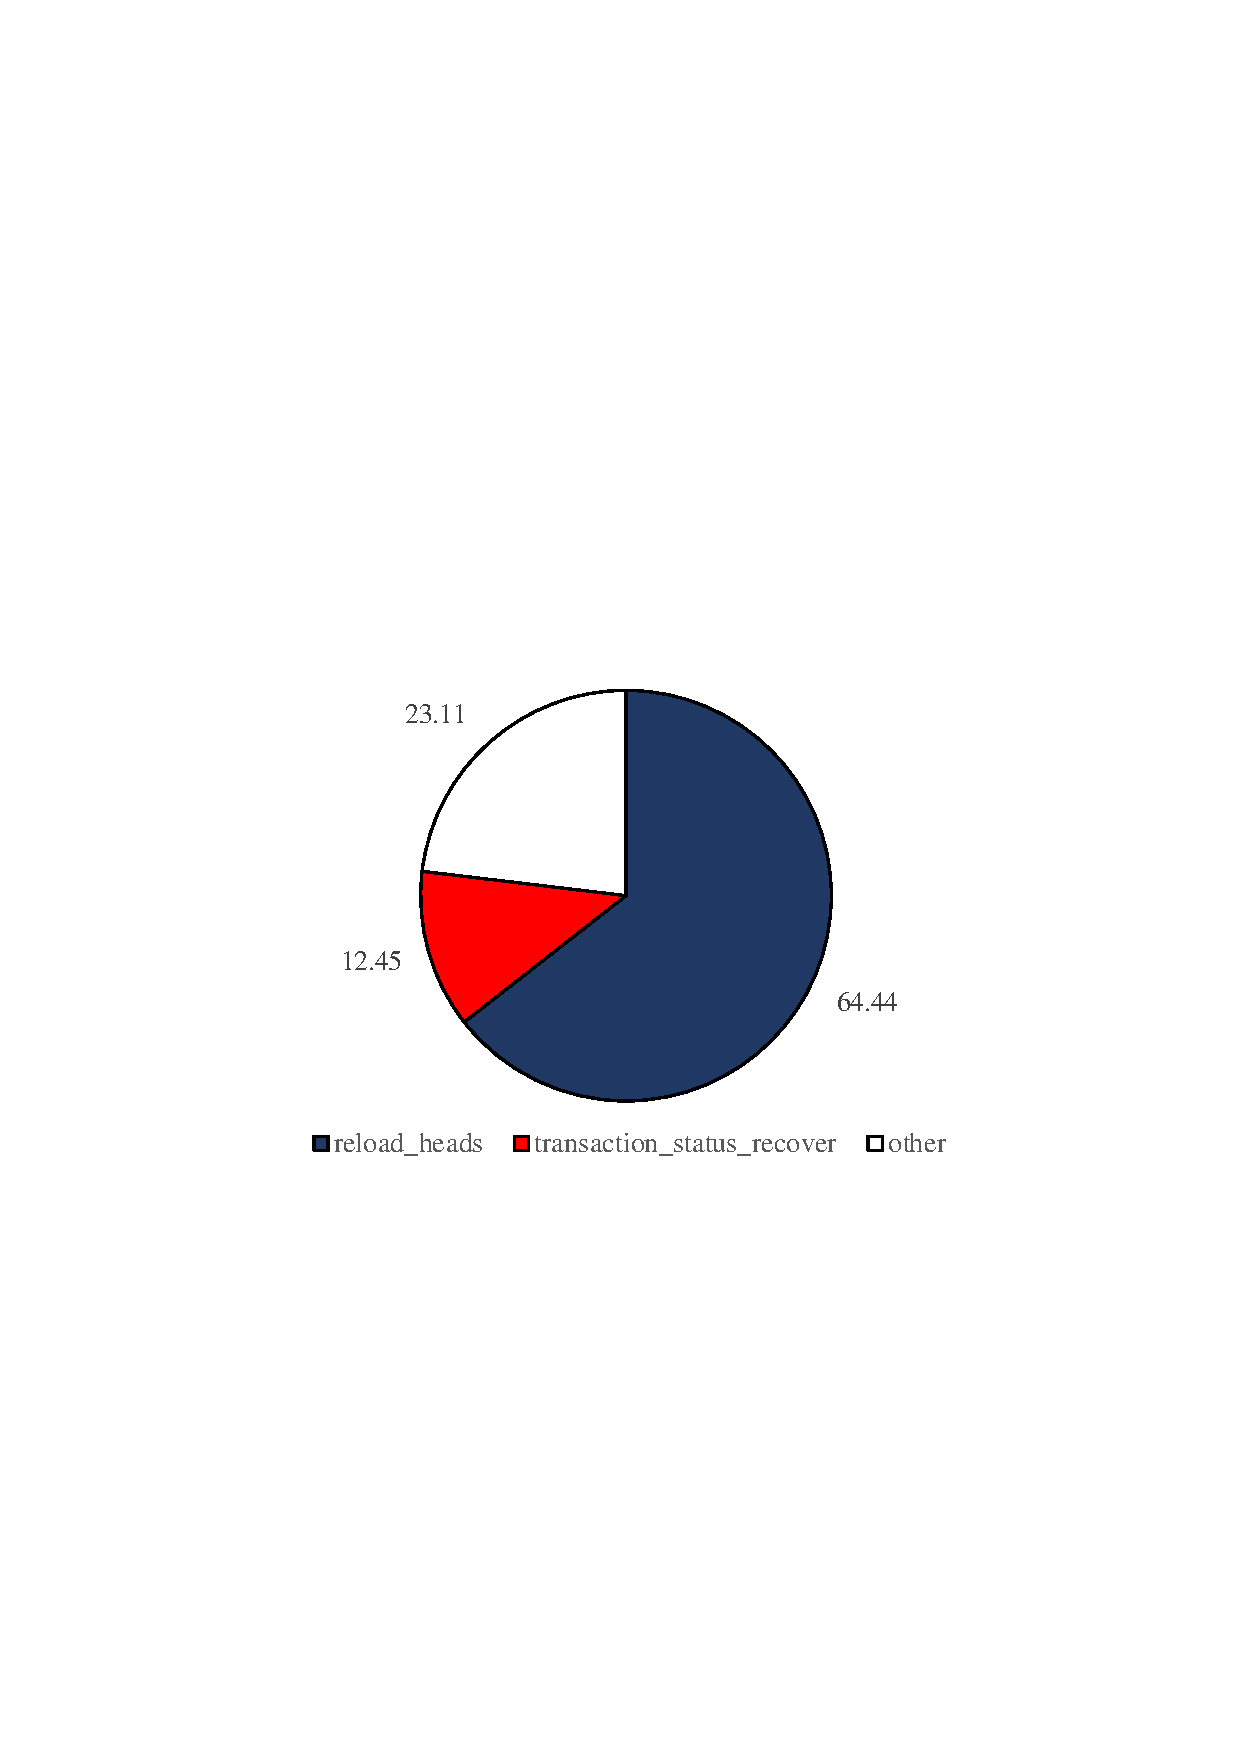
\includegraphics[width=15cm, trim={1cm 9cm 1cm 10cm}]{figures/recovery_perf.pdf}
    \caption{N2DB 的数据恢复性能分析}
    \label{fig:recovery-n2db-perf}
\end{figure}

本章节还分析了两个系统在恢复时的性能分布。
N2DB 的结果展示在图~\ref{fig:recovery-n2db-perf} 中。
从图中可以看出,N2DB 的主要开销在于 reload\_heads。
reload\_heads 的作用是判断所有表格中 head 的可见性。
在目前的实现中,reload\_heads 的开销和表格中 head 的数量成正比。
接下来占比比较大的是事务状态数组的恢复。在数据恢复时系统需要设置之前的事务的状态,将其中未提及的事务的状态设置为 ABORTED。
剩下的元数据恢复以及 NVM 分配器的恢复占了少部分开销。

\begin{figure}
    \centering
    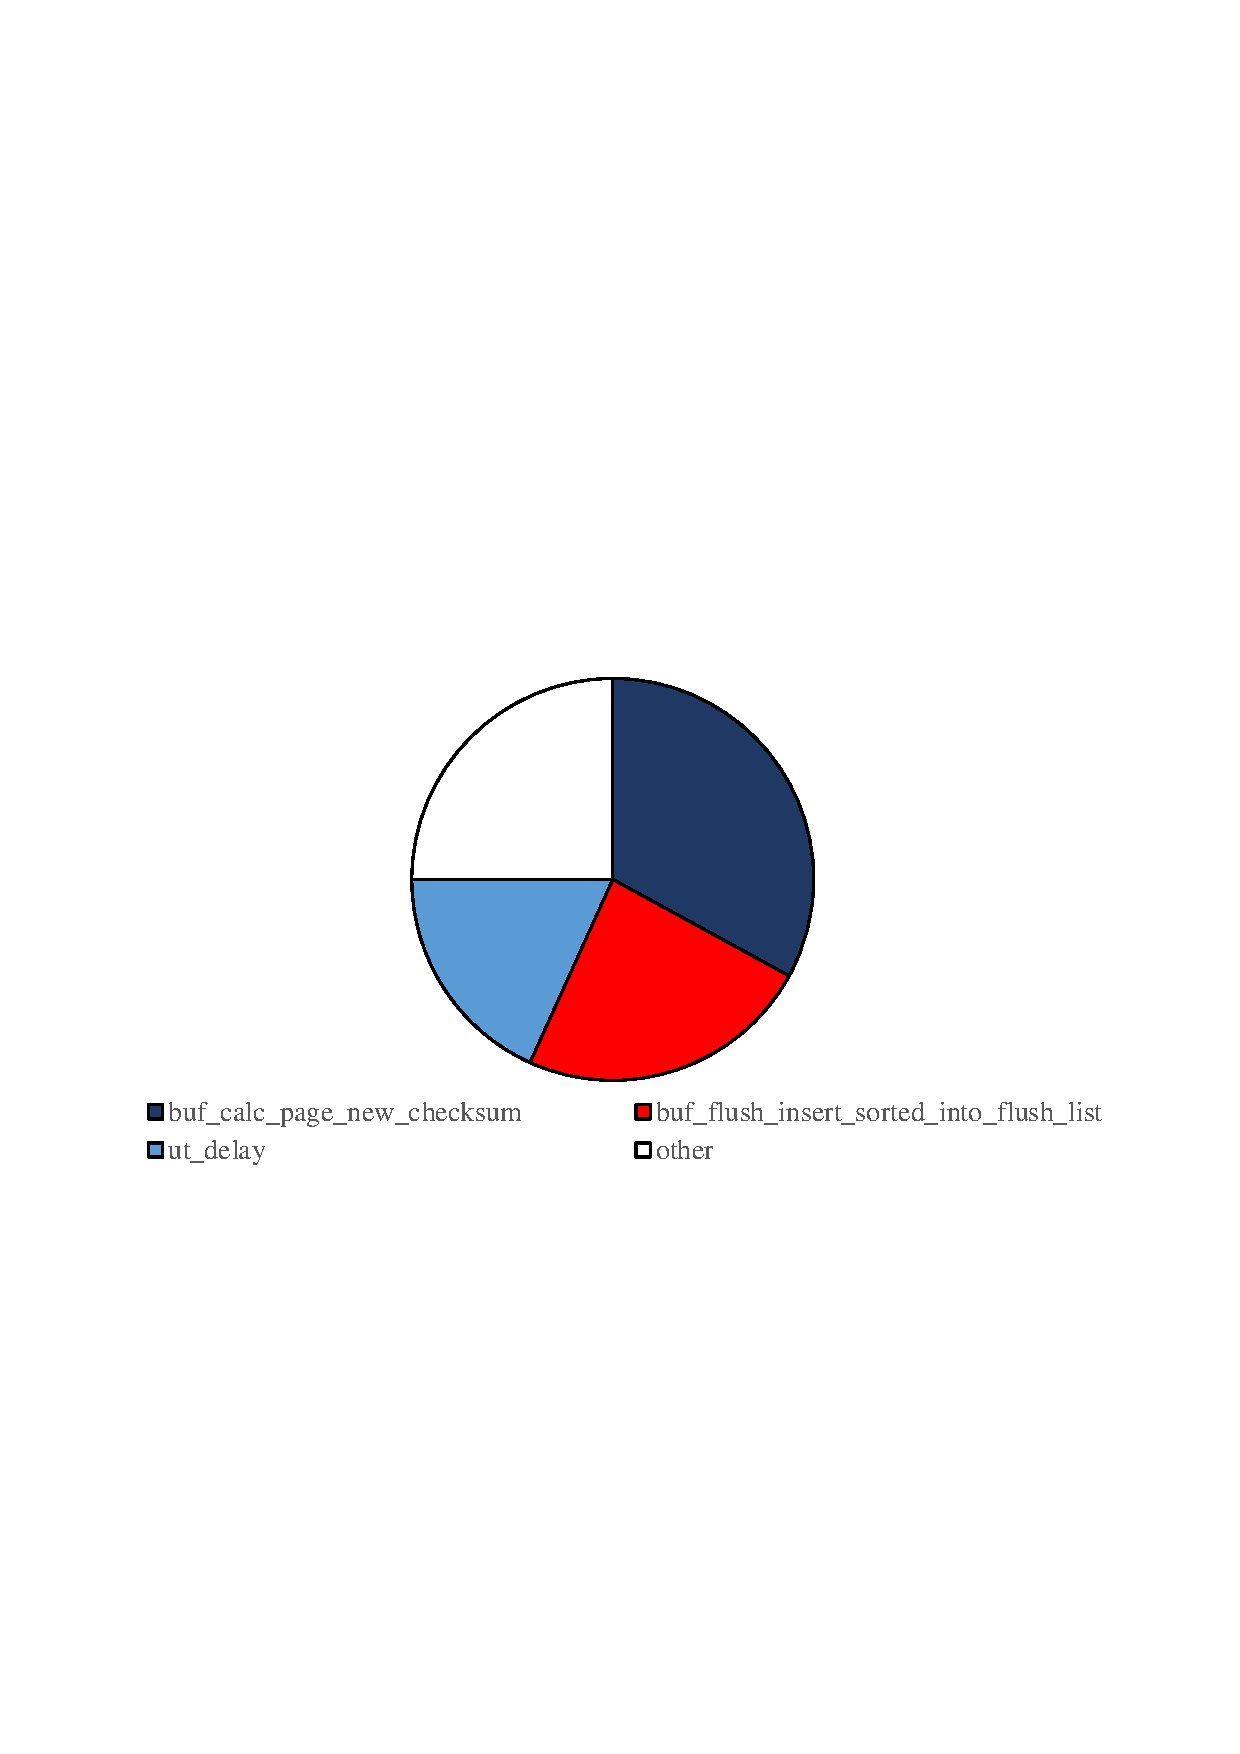
\includegraphics[width=15cm, trim={1cm 9cm 1cm 10cm}]{figures/innodb-recovery-perf.pdf}
    \caption{InnoDB 的数据恢复性能分析}
    \label{fig:recovery-innodb-perf}
\end{figure}


InnoDB 的数据恢复阶段的开销占比如图~\ref{fig:recovery-innodb-perf} 所示。
buf\_flush\_insert\_sorted\_into\_flush\_list 是 InnoDB 在恢复时会调用的数据写回方法。
当 InnoDB 恢复时,其重做阶段和回收阶段都要进行数据的写入。
buf\_calc\_page\_new\_checknum 也是数据写入的一环。
ut\_delay 的开销是由于 InnoDB 在恢复时采用多线程,因此为了避免冲突使用 ut\_delay 来实现自旋锁。

从该开销占比可以看出,InnoDB 在数据恢复阶段的绝大部分开销都是记录数据的修改造成的。
而 N2DB 在数据恢复阶段除了事务状态数组的恢复以外,几乎不需要进行修改操作。
因而 N2DB 的恢复相较于 InnoDB 的 ARIES而言开销极小。








\subsection{存储空间对比}

两个系统的存储空间对比结果展示在图~\ref{fig:recovery-storage-ycsb} 中。
需要注意的是,InnoDB 使用两个日志文件,因此日志的存储空间需要翻倍。
从图中可以看出,N2DB 的存储空间只需要 InnoDB 的一半左右。
主要原因有两点:一是 N2DB 没有日志文件,也不需要存储检查点。
二是相对于 InnoDB 的日志大小,N2DB 的事务状态数组非常轻量。
一百万的事务仅需要 0.2 MB 的存储空间。

\begin{figure}
    \centering
    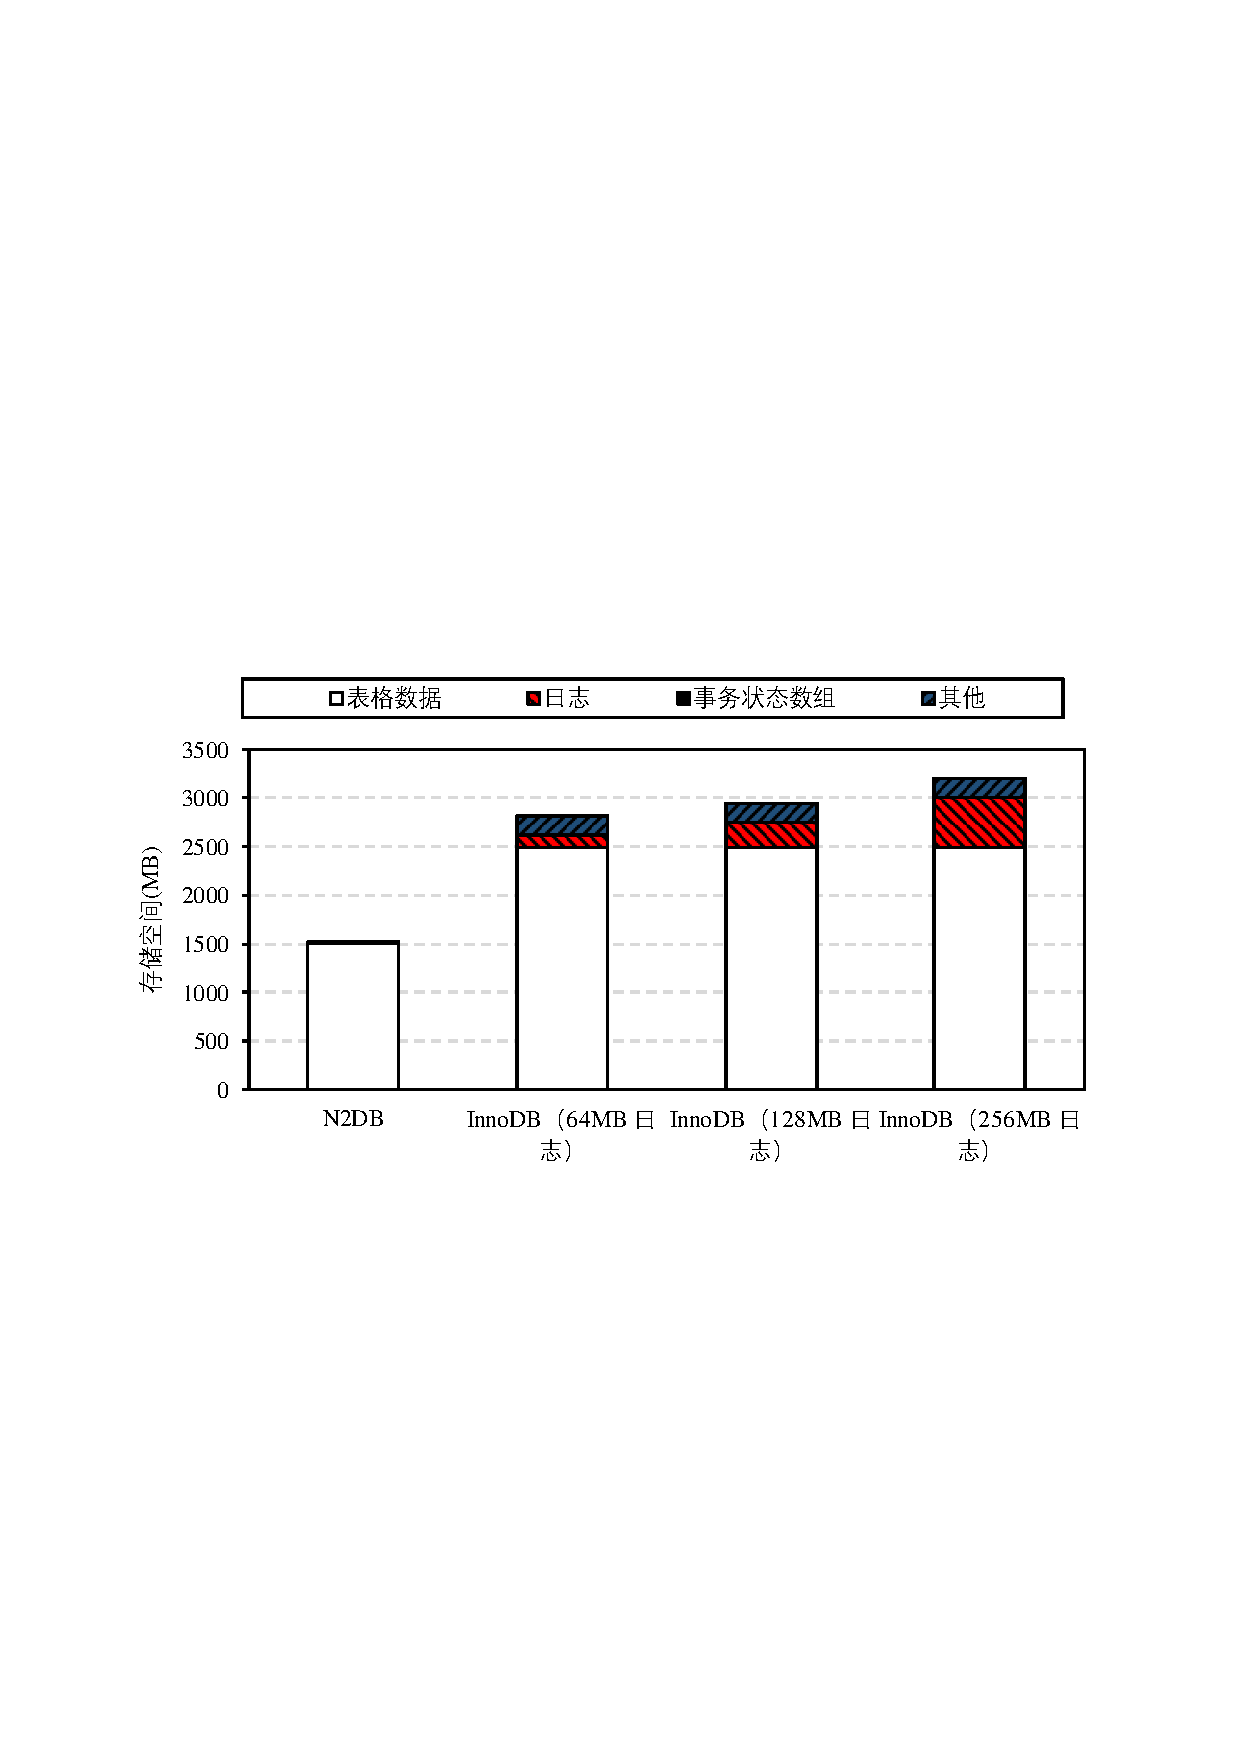
\includegraphics[width=15cm, trim={1cm 9cm 1cm 10cm}]{figures/recovery-storage.pdf}
    \caption{YCSB 负载下垃圾回收性能的存储空间对比实验}
    \label{fig:recovery-storage-ycsb}
\end{figure}



\section{本章小结}

本章节主要对 N2DB 中的垃圾回收机制以及数据恢复机制进行实验,并且对结果进行评估和分析。

首先是垃圾回收机制的性能对比。本章节使用了三种 YCSB 负载以及一种 TPC-C 负载进行测试。相对于关闭垃圾回收的系统,开启垃圾回收的系统在运行时的性能至多降低 $10\%$。但是垃圾回收机制会显著减少存储空间的使用,减少的效果随着事务的更新操作的比例而提升,最高降低 $60\%$ 的存储空间使用。

然后是数据恢复机制的性能对比。实验使用统一的负载以及两种不同的提交事务的阈值。
在两种实验设置中,N2DB 的恢复时间是 InnoDB 的三个数量以下。同时 N2DB 相对于 InnoDB 而言,能够节约 $50\%$ 的存储空间。

综上所述,N2DB 能够在无日志的前提下做到高速地正确地恢复,同时能够有效地利用存储空间,降低对于 NVM 介质的损伤,以保护 NVM 介质的寿命。


%% !TeX root = ../thuthesis-caishiyu.tex

\chapter{相关工作}

\section{NVM 分配器}

\section{NVM 事务内存}

\section{NVM 数据库的日志系统}
% !TeX root = ../thuthesis-caishiyu.tex

\chapter{总结与展望}

\section{本文工作总结}


数据库管理系统是广泛使用的计算机软件。传统的数据库管理系统使用内存-持久化存储介质的双层存储架构,一层作为高速的数据易失的缓存,一层作为大容量的数据存储介质。

非易失性内存是结合内存以及固态硬盘的优点。其作为一个新兴的存储介质给数据库管理系统的研究提供了新的方向。
NVM 优异的硬件特性允许 DBMS 采用单层的存储架构,避免了运行时的复杂的数据管理开销以及频繁的数据同步,进而提高了系统的性能,降低了单个事务的延迟。
N2DB 是第一个零拷贝,无日志的数据库管理系统。
无日志的特性将是 NVM 数据库的一大趋势。

垃圾回收以及数据恢复是基于 NVM 的数据库管理系统中重要的组件。
垃圾回收机制负责回收 NVM 介质上冗余的数据,以最大化利用 NVM 存储空间。
数据恢复机制让 DBMS 从故障中恢复到可工作的状态。
数据恢复机制需要保证系统满足 ACID 四个特性。
然而无日志的前提给数据库的垃圾回收机制以及数据恢复机制带来了挑战。
并且传统的垃圾回收机制以及数据恢复机制难以迁移到 NVM 数据库上。
因此本文在 N2DB 中设计并实现了不基于日志的垃圾回收机制以及数据恢复机制。

本文为了克服 NVM 上编程的挑战,结合 NVM 相关工作使用了 3 个设计方法,树状数据结构,懒惰垃圾回收以及可见性判断。
本文在 Intel Optane DC PMM 环境下测试了两种机制的效果。实验表明,垃圾回收机制能够在至多降低 $10\%$ 的运行时性能的前提下,帮助系统节约至多 $67\%$ 的存储空间。同时与 InnoDB 的恢复性能对比实验表明,本文所提出的无日志数据恢复机制的恢复时间比基于写前日志的恢复时间低至多三个数量级。并且该数据恢复机制节约了一半的存储空间。

本文提出的垃圾回收机制和数据恢复机制可以为其他无日志的数据库管理系统的设计提供参考。
其他的 NVM 数据管理系统只要将事务状态持久化并且将数据结构设计成树状结构,就能采用本文的垃圾回收机制以及数据恢复机制,进而实现高速的容灾恢复。


\section{不足之处和未来研究方向}

截止目前,本文所实现的垃圾机制以及数据恢复机制主要有两个不足之处。
一是垃圾回收机制的开销大,并且没有考虑事务长时间运行对于垃圾回收的阻塞问题。
二是数据恢复的恢复时间还没达到理论上的极限。
现有工作仍需要扫描所有表格的 head,该扫描工作占据了系统恢复的大部分开销。

这两个不足之处是本文未来的工作方向。N2DB 可以采用 Hyper 类似的存储结构,将事务的前像存储在连续的物理空间中,并且一次性回收。采用这样的存储架构理论上能够降低垃圾回收的开销,但是需要针对四种可回收的对象具体分析。
系统需要设计更多的版本相关的操作才能在不影响长时间运行的版本的前提下回收其他可回收空间。
另外 N2DB 可以通过实现持久化索引来降低重启之后的开销。理论上可以通过设计索引的节点的可见性来实现即刻恢复的数据恢复机制,但是持久化索引相对于内存中的索引的读性能较低,可能会影响事务的吞吐率。




% 其他部分
\backmatter

% 参考文献
\bibliography{ref/refs}  % 参考文献使用 BibTeX 编译
% \printbibliography       % 参考文献使用 BibLaTeX 编译

% 附录
\appendix
% \chapter{补充内容}

附录是与论文内容密切相关、但编入正文又影响整篇论文编排的条理和逻辑性的资料,例如某些重要的数据表格、计算程序、统计表等,是论文主体的补充内容,可根据需要设置。


\section{图表示例}

\subsection{图}

附录中的图片示例(图~\ref{fig:appendix-figure})。

\begin{figure}
  \centering
  
\includegraphics[width=0.6\linewidth]{example-image-a.pdf}
  \caption{附录中的图片示例}
  \label{fig:appendix-figure}
\end{figure}


\subsection{表格}

附录中的表格示例(表~\ref{tab:appendix-table})。

\begin{table}
  \centering
  \caption{附录中的表格示例}
  \begin{tabular}{ll}
    \toprule
    文件名          & 描述                         \\
    \midrule
    thuthesis.dtx   & 模板的源文件,包括文档和注释 \\
    thuthesis.cls   & 模板文件                     \\
    thuthesis-*.bst & BibTeX 参考文献表样式文件    \\
    thuthesis-*.bbx & BibLaTeX 参考文献表样式文件  \\
    thuthesis-*.cbx & BibLaTeX 引用样式文件        \\
    \bottomrule
  \end{tabular}
  \label{tab:appendix-table}
\end{table}


\section{数学公式}

附录中的数学公式示例(公式~\eqref{eq:appendix-equation})。
\begin{equation}
  \frac{1}{2 \symup{\pi} \symup{i}} \int_\gamma f = \sum_{k=1}^m n(\gamma; a_k) \mathscr{R}(f; a_k)
  \label{eq:appendix-equation}
\end{equation}

% % !TeX root = ../thuthesis-example.tex

\begin{survey}
\label{cha:survey}

\title{Title of the Survey}
\maketitle


\tableofcontents


本科生的外文资料调研阅读报告。


\section{Figures and Tables}

\subsection{Figures}

An example figure in appendix (Figure~\ref{fig:appendix-survey-figure}).

\begin{figure}
  \centering
  
\includegraphics[width=0.6\linewidth]{example-image-a.pdf}
  \caption{Example figure in appendix}
  \label{fig:appendix-survey-figure}
\end{figure}


\subsection{Tables}

An example table in appendix (Table~\ref{tab:appendix-survey-table}).

\begin{table}
  \centering
  \caption{Example table in appendix}
  \begin{tabular}{ll}
    \toprule
    File name       & Description                                         \\
    \midrule
    thuthesis.dtx   & The source file including documentaion and comments \\
    thuthesis.cls   & The template file                                   \\
    thuthesis-*.bst & BibTeX styles                                       \\
    thuthesis-*.bbx & BibLaTeX styles for bibliographies                  \\
    thuthesis-*.cbx & BibLaTeX styles for citations                       \\
    \bottomrule
  \end{tabular}
  \label{tab:appendix-survey-table}
\end{table}


\section{Equations}

An example equation in appendix (Equation~\eqref{eq:appendix-survey-equation}).
\begin{equation}
  \frac{1}{2 \symup{\pi} \symup{i}} \int_\gamma f = \sum_{k=1}^m n(\gamma; a_k) \mathscr{R}(f; a_k)
  \label{eq:appendix-survey-equation}
\end{equation}


\section{Citations}

Example citations in appendix.
\cite{abrahams99tex}
\cite{salomon1995advanced}
\cite{abrahams99tex,salomon1995advanced}


\bibliographystyle{unsrtnat}
\bibliography{ref/appendix}

\end{survey}
       % 本科生:外文资料的调研阅读报告
% % !TeX root = ../thuthesis-caishiyu.tex

\begin{translation}
\label{cha:translation}

\title{书面翻译题目}
\maketitle

\tableofcontents


本科生的外文资料书面翻译。


\section{图表示例}

\subsection{图}

附录中的图片示例(图~\ref{fig:appendix-translation-figure})。

\begin{figure}
  \centering
  
\includegraphics[width=0.6\linewidth]{example-image-a.pdf}
  \caption{附录中的图片示例}
  \label{fig:appendix-translation-figure}
\end{figure}


\subsection{表格}

附录中的表格示例(表~\ref{tab:appendix-translation-table})。

\begin{table}
  \centering
  \caption{附录中的表格示例}
  \begin{tabular}{ll}
    \toprule
    文件名          & 描述                         \\
    \midrule
    thuthesis.dtx   & 模板的源文件,包括文档和注释 \\
    thuthesis.cls   & 模板文件                     \\
    thuthesis-*.bst & BibTeX 参考文献表样式文件    \\
    thuthesis-*.bbx & BibLaTeX 参考文献表样式文件  \\
    thuthesis-*.cbx & BibLaTeX 引用样式文件        \\
    \bottomrule
  \end{tabular}
  \label{tab:appendix-translation-table}
\end{table}


\section{数学公式}

附录中的数学公式示例(公式~\eqref{eq:appendix-translation-equation})。
\begin{equation}
  \frac{1}{2 \symup{\pi} \symup{i}} \int_\gamma f = \sum_{k=1}^m n(\gamma; a_k) \mathscr{R}(f; a_k)
  \label{eq:appendix-translation-equation}
\end{equation}


\section{文献引用}

文献引用示例\cite{abrahams99tex}。


% 书面翻译的参考文献
\bibliographystyle{unsrtnat}
\bibliography{ref/appendix}

% 书面翻译对应的原文索引
\begin{translation-index}
\nocite{salomon1995advanced}
\bibliographystyle{unsrtnat}
\bibliography{ref/appendix}
\end{translation-index}

\end{translation}
  % 本科生:外文资料的书面翻译

% 致谢
% !TeX root = ../thuthesis-caishiyu.tex

\begin{acknowledgements}
  衷心感谢导师×××教授和物理系××副教授对本人的精心指导。他们的言传身教将使我终生受益。

  在美国麻省理工学院化学系进行九个月的合作研究期间,承蒙 Robert Field 教授热心指导与帮助,不胜感激。

  感谢×××××实验室主任×××教授,以及实验室全体老师和同窗们学的热情帮助和支持!

  本课题承蒙国家自然科学基金资助,特此致谢。
\end{acknowledgements}


% 声明
\statement
% 生成的声明页是否要插入页眉和页脚(默认 empty)
% 仅在需要进行电子签名时,才需要打开这一选项
% 插入的扫描声明页总是会生成页眉(研究生)和页脚,不受这一选项影响
% \statement[page-style=plain]
% 将签字扫描后的声明文件 scan-statement.pdf 替换原始页面
% \statement[file=scan-statement.pdf]

% 个人简历、在学期间完成的相关学术成果
% !TeX root = ../thuthesis-caishiyu.tex

\begin{resume}

  \section*{个人简历}

  197× 年 ×× 月 ×× 日出生于四川××县。

  1992 年 9 月考入××大学化学系××化学专业,1996 年 7 月本科毕业并获得理学学士学位。

  1996 年 9 月免试进入清华大学化学系攻读××化学博士至今。


  \section*{在学期间完成的相关学术成果}

  \subsection*{学术论文}

  \begin{achievements}
    \item Yang Y, Ren T L, Zhang L T, et al. Miniature microphone with silicon-based ferroelectric thin films[J]. Integrated Ferroelectrics, 2003, 52:229-235.
    \item 杨轶, 张宁欣, 任天令, 等. 硅基铁电微声学器件中薄膜残余应力的研究[J]. 中国机械工程, 2005, 16(14):1289-1291.
    \item 杨轶, 张宁欣, 任天令, 等. 集成铁电器件中的关键工艺研究[J]. 仪器仪表学报, 2003, 24(S4):192-193.
    \item Yang Y, Ren T L, Zhu Y P, et al. PMUTs for handwriting recognition. In press[J]. (已被Integrated Ferroelectrics录用)
  \end{achievements}


  \subsection*{专利}

  \begin{achievements}
    \item 任天令, 杨轶, 朱一平, 等. 硅基铁电微声学传感器畴极化区域控制和电极连接的方法: 中国, CN1602118A[P]. 2005-03-30.
    \item Ren T L, Yang Y, Zhu Y P, et al. Piezoelectric micro acoustic sensor based on ferroelectric materials: USA, No.11/215, 102[P]. (美国发明专利申请号.)
  \end{achievements}

\end{resume}


% 指导教师/指导小组学术评语
% !TeX root = ../thuthesis-caishiyu.tex

\chapter{指导小组学术评语}

论文提出了……


% 答辩委员会决议书
% !TeX root = ../thuthesis-caishiyu.tex

\chapter{答辩委员会决议书}

论文提出了……

论文取得的主要创新性成果包括:

1. ……

2. ……

3. ……

论文工作表明作者在×××××具有×××××知识,具有××××能力,论文××××,答辩××××。

答辩委员会表决,(×票/一致)同意通过论文答辩,并建议授予×××(姓名)×××(门类)学博士/硕士学位。


% 本科生的综合论文训练记录表(扫描版)
% \record{file=scan-record.pdf}

\end{document}
